\documentclass[11pt,preprint]{elsarticle}

\usepackage{lmodern}
%%%% My spacing
\usepackage{setspace}
\setstretch{1.2}
\DeclareMathSizes{12}{14}{10}{10}

% Wrap around which gives all figures included the [H] command, or places it "here". This can be tedious to code in Rmarkdown.
\usepackage{float}
\let\origfigure\figure
\let\endorigfigure\endfigure
\renewenvironment{figure}[1][2] {
    \expandafter\origfigure\expandafter[H]
} {
    \endorigfigure
}

\let\origtable\table
\let\endorigtable\endtable
\renewenvironment{table}[1][2] {
    \expandafter\origtable\expandafter[H]
} {
    \endorigtable
}


\usepackage{ifxetex,ifluatex}
\usepackage{fixltx2e} % provides \textsubscript
\ifnum 0\ifxetex 1\fi\ifluatex 1\fi=0 % if pdftex
  \usepackage[T1]{fontenc}
  \usepackage[utf8]{inputenc}
\else % if luatex or xelatex
  \ifxetex
    \usepackage{mathspec}
    \usepackage{xltxtra,xunicode}
  \else
    \usepackage{fontspec}
  \fi
  \defaultfontfeatures{Mapping=tex-text,Scale=MatchLowercase}
  \newcommand{\euro}{€}
\fi

\usepackage{amssymb, amsmath, amsthm, amsfonts}

\def\bibsection{\section*{References}} %%% Make "References" appear before bibliography


\usepackage[numbers]{natbib}

\usepackage{longtable}
\usepackage[margin=2.3cm,bottom=2cm,top=2.5cm, includefoot]{geometry}
\usepackage{fancyhdr}
\usepackage[bottom, hang, flushmargin]{footmisc}
\usepackage{graphicx}
\numberwithin{equation}{section}
\numberwithin{figure}{section}
\numberwithin{table}{section}
\setlength{\parindent}{0cm}
\setlength{\parskip}{1.3ex plus 0.5ex minus 0.3ex}
\usepackage{textcomp}
\renewcommand{\headrulewidth}{0.2pt}
\renewcommand{\footrulewidth}{0.3pt}

\usepackage{array}
\newcolumntype{x}[1]{>{\centering\arraybackslash\hspace{0pt}}p{#1}}

%%%%  Remove the "preprint submitted to" part. Don't worry about this either, it just looks better without it:
\makeatletter
\def\ps@pprintTitle{%
  \let\@oddhead\@empty
  \let\@evenhead\@empty
  \let\@oddfoot\@empty
  \let\@evenfoot\@oddfoot
}
\makeatother

 \def\tightlist{} % This allows for subbullets!

\usepackage{hyperref}
\hypersetup{breaklinks=true,
            bookmarks=true,
            colorlinks=true,
            citecolor=blue,
            urlcolor=blue,
            linkcolor=blue,
            pdfborder={0 0 0}}


% The following packages allow huxtable to work:
\usepackage{siunitx}
\usepackage{multirow}
\usepackage{hhline}
\usepackage{calc}
\usepackage{tabularx}
\usepackage{booktabs}
\usepackage{caption}


\newenvironment{columns}[1][]{}{}

\newenvironment{column}[1]{\begin{minipage}{#1}\ignorespaces}{%
\end{minipage}
\ifhmode\unskip\fi
\aftergroup\useignorespacesandallpars}

\def\useignorespacesandallpars#1\ignorespaces\fi{%
#1\fi\ignorespacesandallpars}

\makeatletter
\def\ignorespacesandallpars{%
  \@ifnextchar\par
    {\expandafter\ignorespacesandallpars\@gobble}%
    {}%
}
\makeatother


% definitions for citeproc citations
\NewDocumentCommand\citeproctext{}{}
\NewDocumentCommand\citeproc{mm}{%
\href{\#cite.\detokenize{#1}}{#2}\nocite{#1}}

\makeatletter
% allow citations to break across lines
\let\@cite@ofmt\@firstofone
% avoid brackets around text for \cite:
\def\@biblabel#1{}
\def\@cite#1#2{{#1\if@tempswa , #2\fi}}
\makeatother
\newlength{\cslhangindent}
\setlength{\cslhangindent}{1.5em}
\newlength{\csllabelwidth}
\setlength{\csllabelwidth}{3em}
\newenvironment{CSLReferences}[2] % #1 hanging-indent, #2 entry-spacing
{\begin{list}{}{%
	\setlength{\itemindent}{0pt}
	\setlength{\leftmargin}{0pt}
	\setlength{\parsep}{0pt}
	% turn on hanging indent if param 1 is 1
	\ifodd #1
	\setlength{\leftmargin}{\cslhangindent}
	\setlength{\itemindent}{-1\cslhangindent}
	\fi
	% set entry spacing
	\setlength{\itemsep}{#2\baselineskip}}}
{\end{list}}

\usepackage{calc}
\newcommand{\CSLBlock}[1]{\hfill\break\parbox[t]{\linewidth}{\strut\ignorespaces#1\strut}}
\newcommand{\CSLLeftMargin}[1]{\parbox[t]{\csllabelwidth}{\strut#1\strut}}
\newcommand{\CSLRightInline}[1]{\parbox[t]{\linewidth - \csllabelwidth}{\strut#1\strut}}
\newcommand{\CSLIndent}[1]{\hspace{\cslhangindent}#1}


\urlstyle{same}  % don't use monospace font for urls
\setlength{\parindent}{0pt}
\setlength{\parskip}{6pt plus 2pt minus 1pt}
\setlength{\emergencystretch}{3em}  % prevent overfull lines
\setcounter{secnumdepth}{5}

%%% Use protect on footnotes to avoid problems with footnotes in titles
\let\rmarkdownfootnote\footnote%
\def\footnote{\protect\rmarkdownfootnote}
\IfFileExists{upquote.sty}{\usepackage{upquote}}{}

%%% Include extra packages specified by user
\newcounter{none}
\usepackage{colortbl}\usepackage{booktabs}
\usepackage{longtable}
\usepackage{array}
\usepackage{multirow}
\usepackage{wrapfig}
\usepackage{float}
\usepackage{colortbl}
\usepackage{pdflscape}
\usepackage{tabu}
\usepackage{threeparttable}
\usepackage{threeparttablex}
\usepackage[normalem]{ulem}
\usepackage{makecell}
\usepackage{xcolor}

%%% Hard setting column skips for reports - this ensures greater consistency and control over the length settings in the document.
%% page layout
%% paragraphs
\setlength{\baselineskip}{12pt plus 0pt minus 0pt}
\setlength{\parskip}{12pt plus 0pt minus 0pt}
\setlength{\parindent}{0pt plus 0pt minus 0pt}
%% floats
\setlength{\floatsep}{12pt plus 0 pt minus 0pt}
\setlength{\textfloatsep}{20pt plus 0pt minus 0pt}
\setlength{\intextsep}{14pt plus 0pt minus 0pt}
\setlength{\dbltextfloatsep}{20pt plus 0pt minus 0pt}
\setlength{\dblfloatsep}{14pt plus 0pt minus 0pt}
%% maths
\setlength{\abovedisplayskip}{12pt plus 0pt minus 0pt}
\setlength{\belowdisplayskip}{12pt plus 0pt minus 0pt}
%% lists
\setlength{\topsep}{10pt plus 0pt minus 0pt}
\setlength{\partopsep}{3pt plus 0pt minus 0pt}
\setlength{\itemsep}{5pt plus 0pt minus 0pt}
\setlength{\labelsep}{8mm plus 0mm minus 0mm}
\setlength{\parsep}{\the\parskip}
\setlength{\listparindent}{\the\parindent}
%% verbatim
\setlength{\fboxsep}{5pt plus 0pt minus 0pt}



\begin{document}



\begin{frontmatter}  %

\title{Global Volatility Report}

% Set to FALSE if wanting to remove title (for submission)




\author[Add1]{Martin Raubenheimer24954578}
\ead{martinraubs@gmail.com}





\address[Add1]{Department of Economics, Stellenbosch University, South
Africa}



\vspace{1cm}





\vspace{0.5cm}

\end{frontmatter}

\setcounter{footnote}{0}



%________________________
% Header and Footers
%%%%%%%%%%%%%%%%%%%%%%%%%%%%%%%%%
\pagestyle{fancy}
\chead{}
\rhead{}
\lfoot{}
\rfoot{\footnotesize Page \thepage}
\lhead{}
%\rfoot{\footnotesize Page \thepage } % "e.g. Page 2"
\cfoot{}

%\setlength\headheight{30pt}
%%%%%%%%%%%%%%%%%%%%%%%%%%%%%%%%%
%________________________

\headsep 35pt % So that header does not go over title




\section{Part A: How has volatility
increased?}\label{part-a-how-has-volatility-increased}

\subsection{Global implied volatility}\label{global-implied-volatility}

\begin{itemize}
\tightlist
\item
  The VIX, V2X and VXEEM move closely together, so global volatility is
  highly synchronised.
\item
  The largest spikes were the GFC (V2X above 110) and COVID in 2020 (V2X
  and VXEEM above 90).
\item
  Smaller spikes followed in 2022, early 2025 (VIX around 50) and 2026.
  The 2026 spike was largest in emerging markets (VXEEM mid-40s).
\item
  Since 2023 the indices have mostly sat between 15 and 25.
\item
  Volatility is episodic and mean-reverting. Recent spikes are well
  below the GFC and COVID, so there is no sustained structural increase.
\end{itemize}

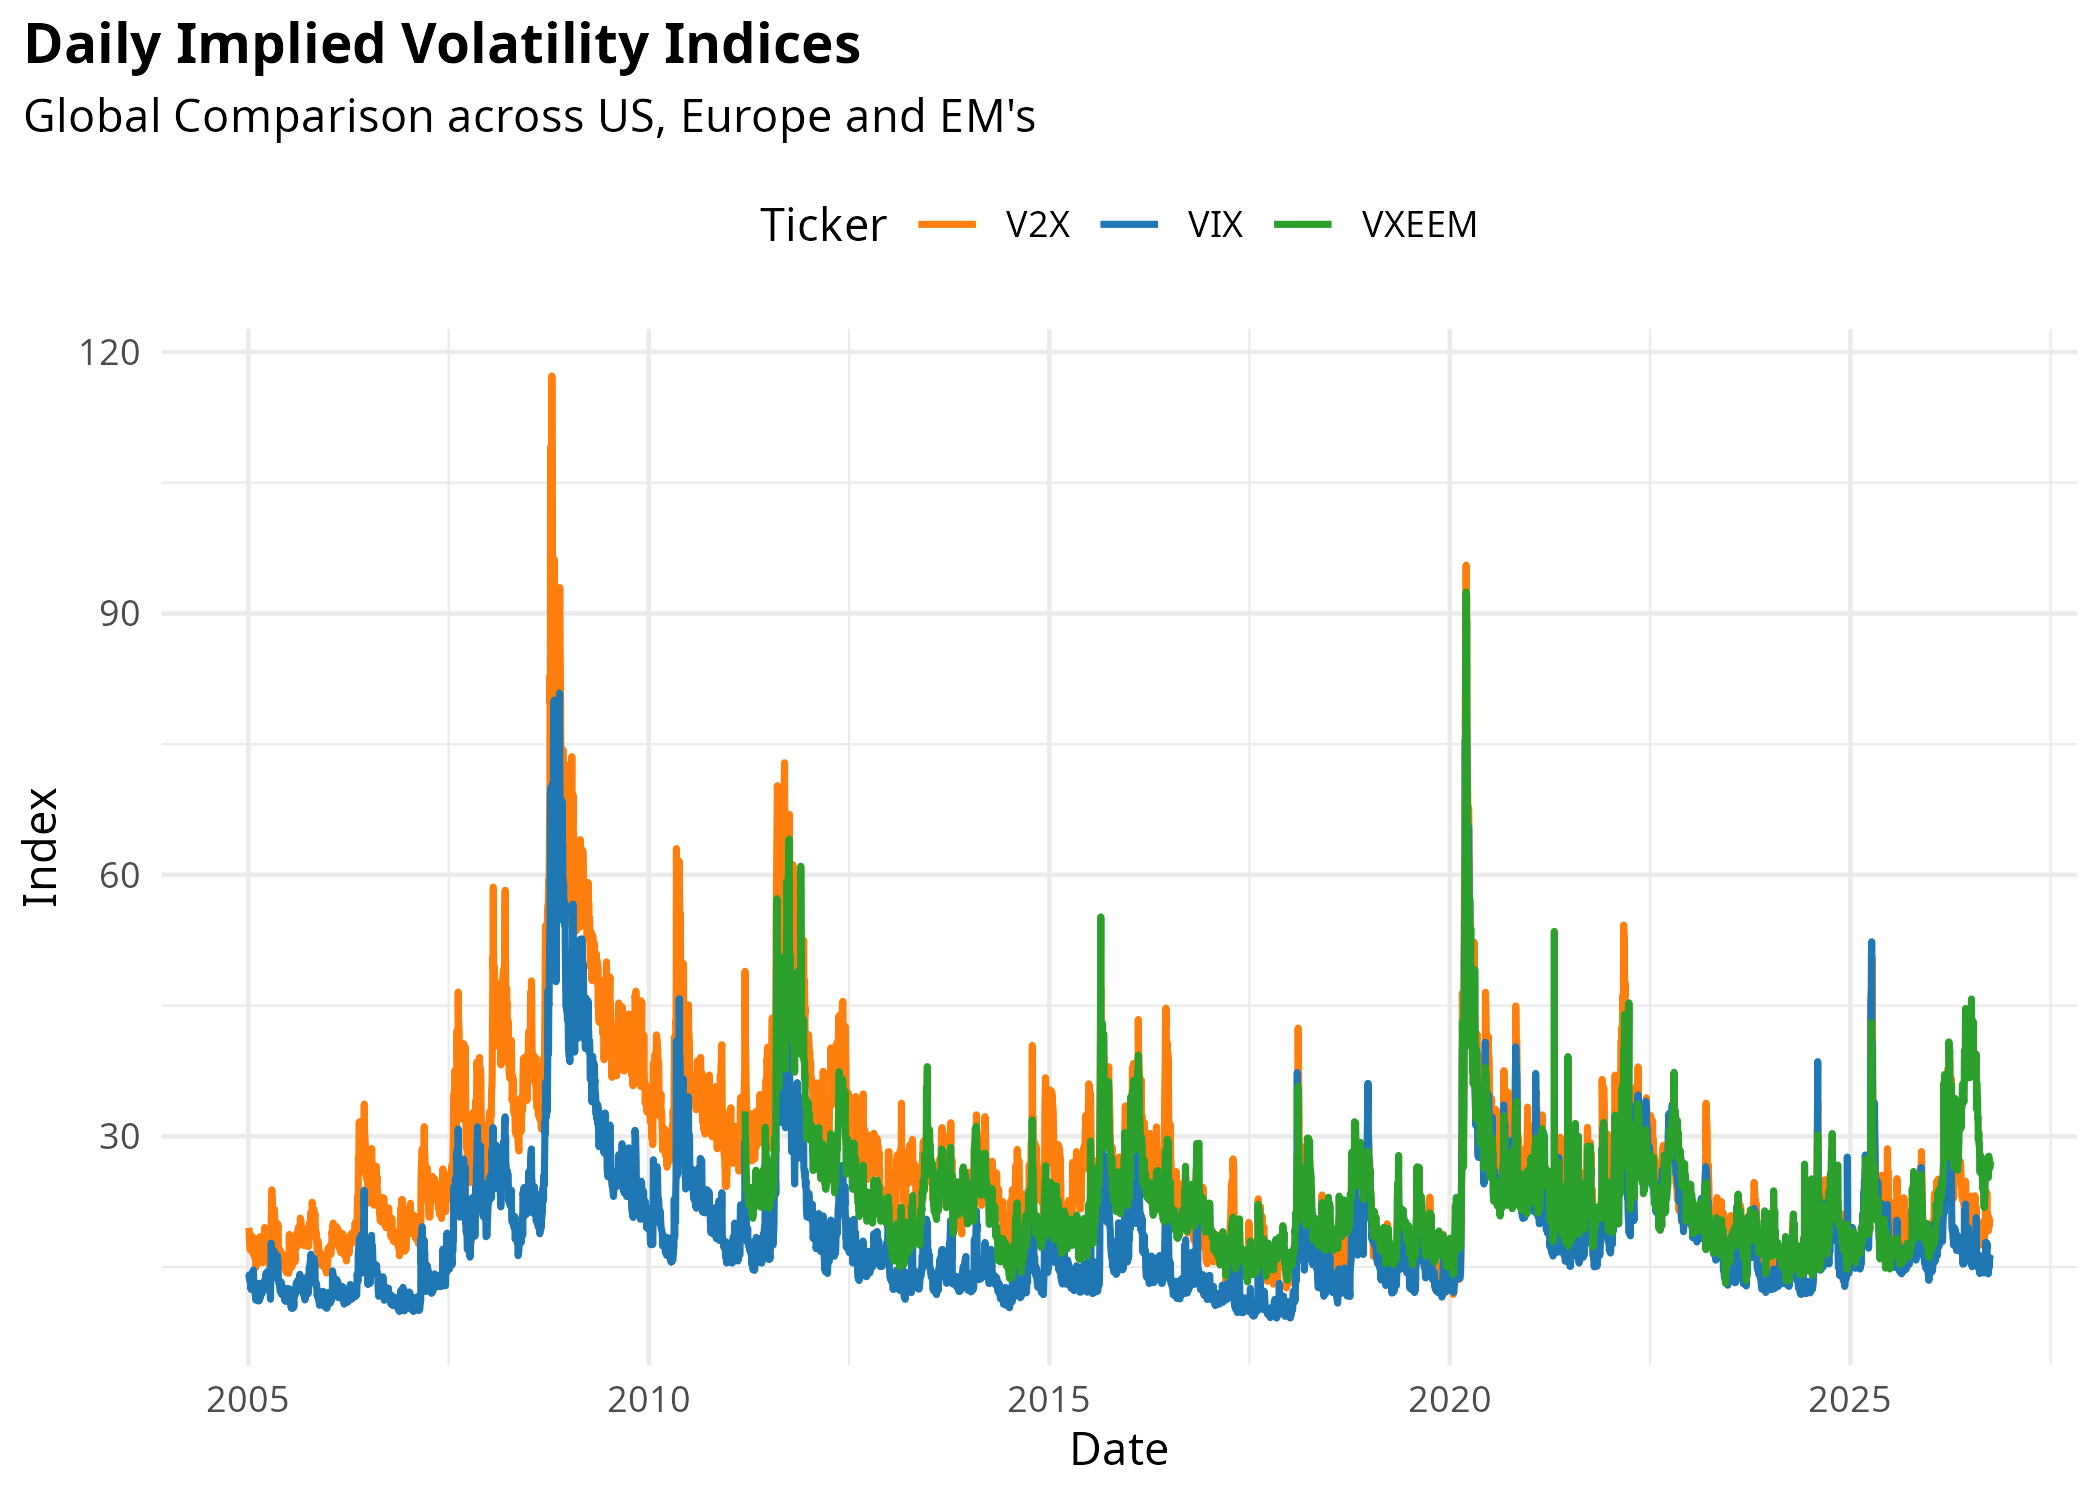
\includegraphics[width=1\linewidth]{figures/Implied_Vol_Plot}

\subsection{Daily returns}\label{daily-returns}

\begin{itemize}
\tightlist
\item
  Returns show volatility clustering: calm periods are interrupted by
  clusters of large moves.
\item
  The largest daily moves were in March 2020 (roughly ±8--10\%). Recent
  large down days of about 5--6\% occurred in 2025 and 2026.
\item
  The pattern is similar across the JSE indices (J200, J201, J202, J433)
  and the Capped SWIX style indices.
\end{itemize}

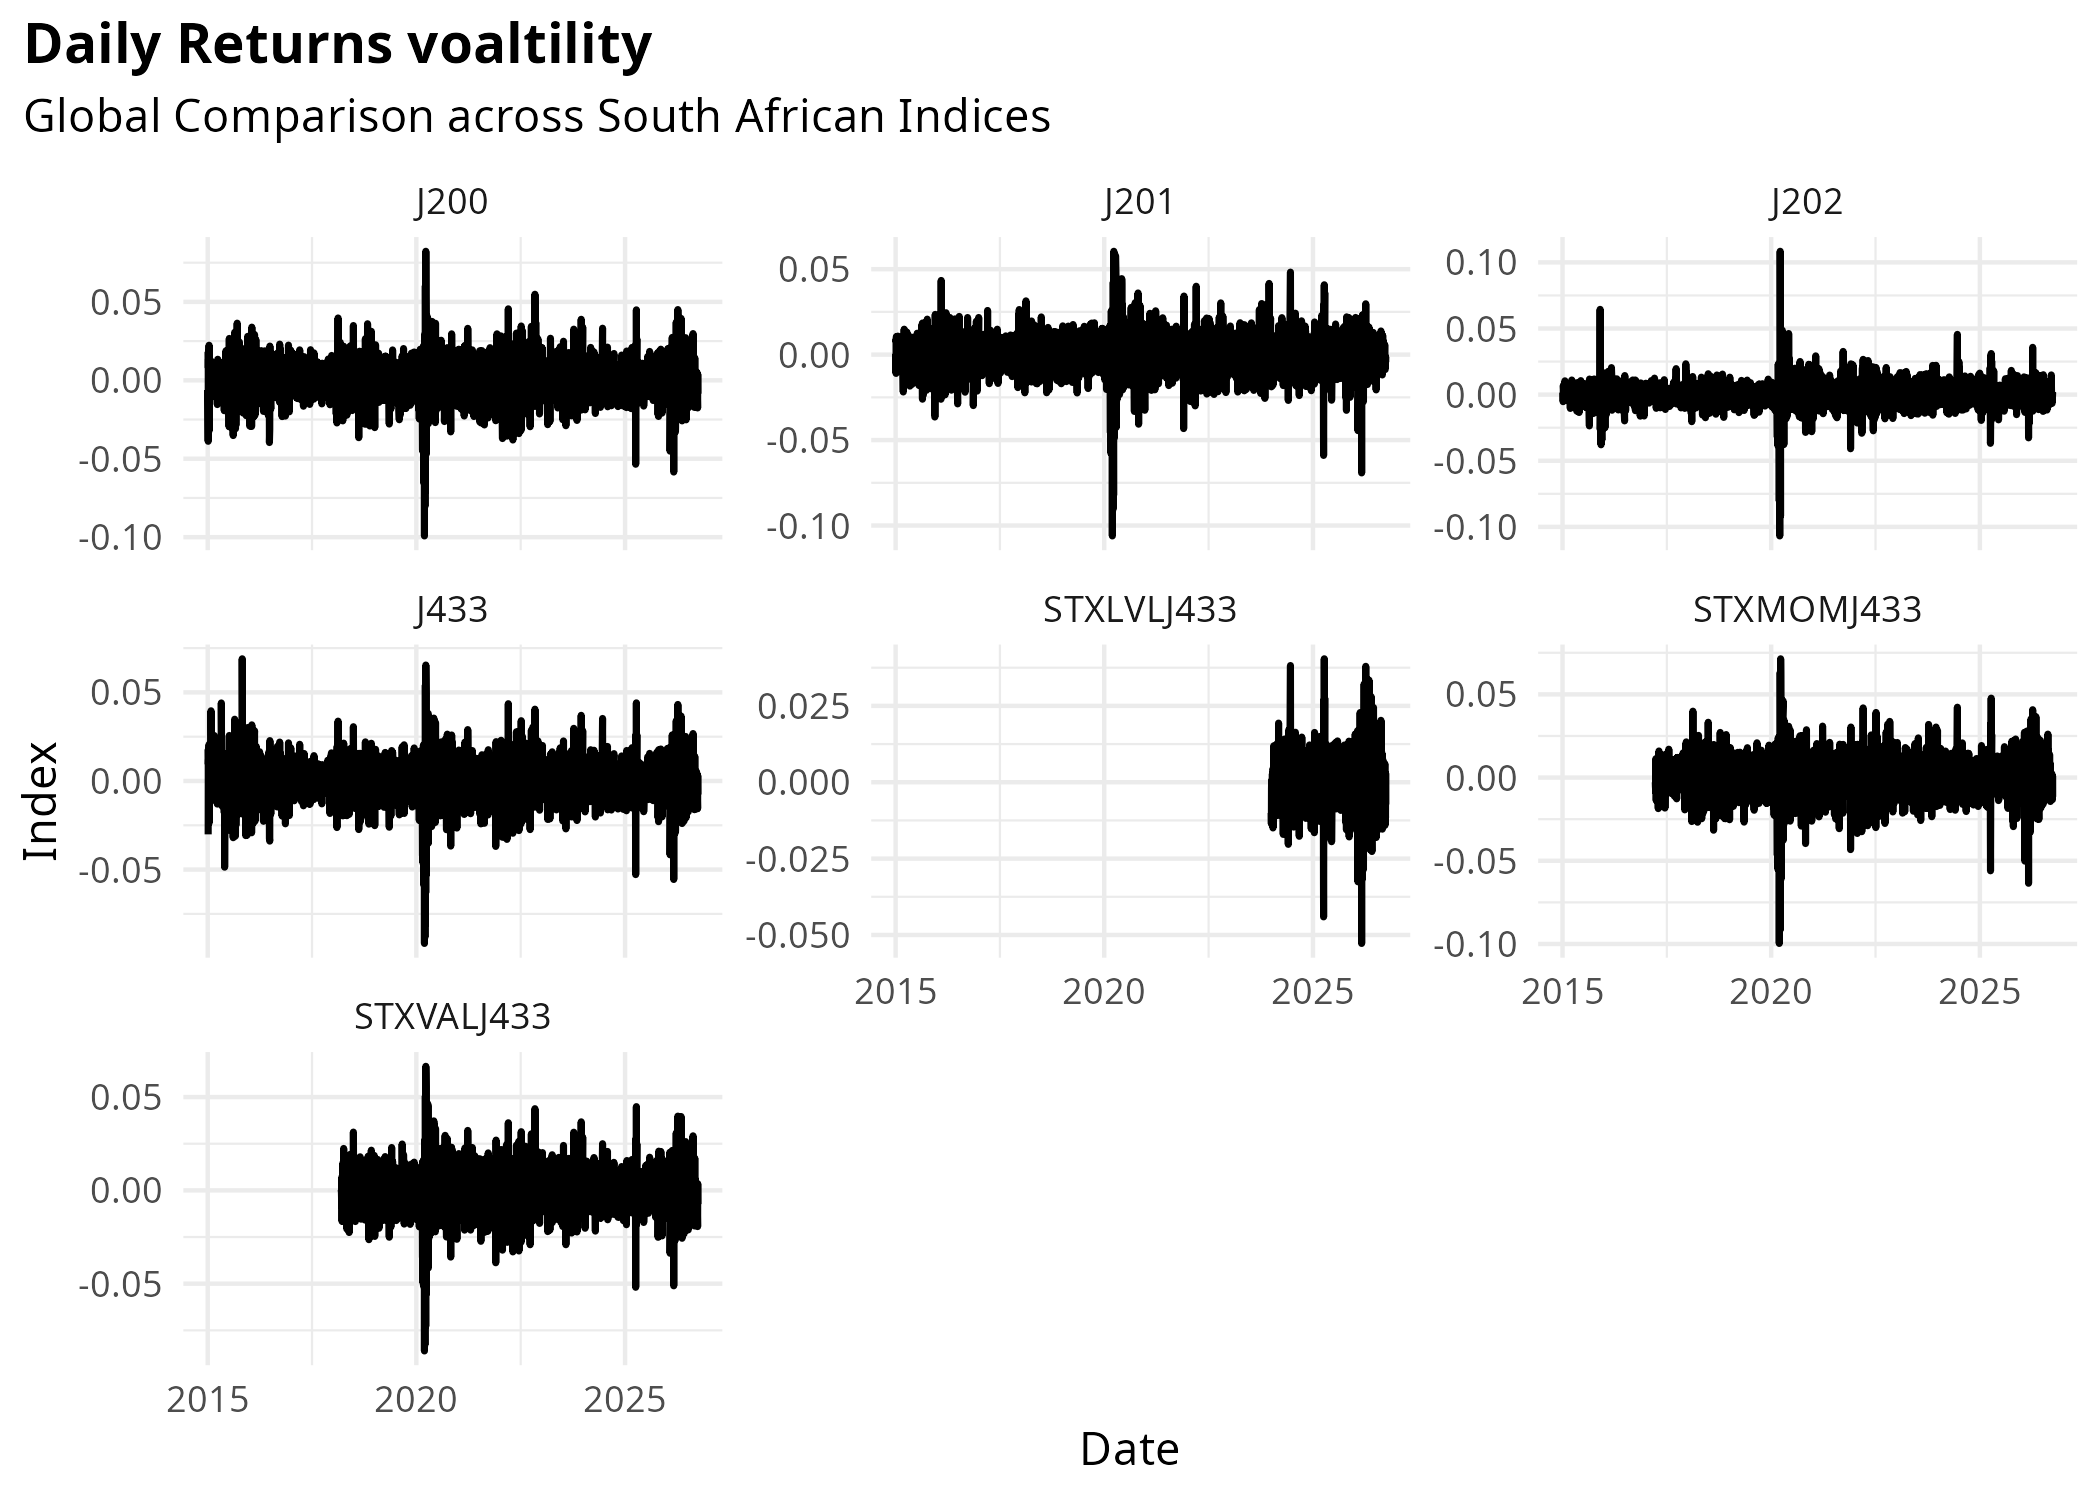
\includegraphics[width=1\linewidth]{figures/abs_return_plot}

\subsection{Rolling volatility}\label{rolling-volatility}

\begin{itemize}
\tightlist
\item
  The 120-day annualised volatility of SA indices usually sits between
  10\% and 20\%.
\item
  It peaked at about 40--43\% in 2020, with smaller episodes in 2016,
  2022 and 2025--26 (roughly 20--26\%).
\item
  All indices rise together, and the style indices track the J433
  closely. J202 is generally the least volatile.
\item
  SA volatility is currently elevated compared with 2023--24 but far
  below 2020, so it is not trending upward.
\end{itemize}

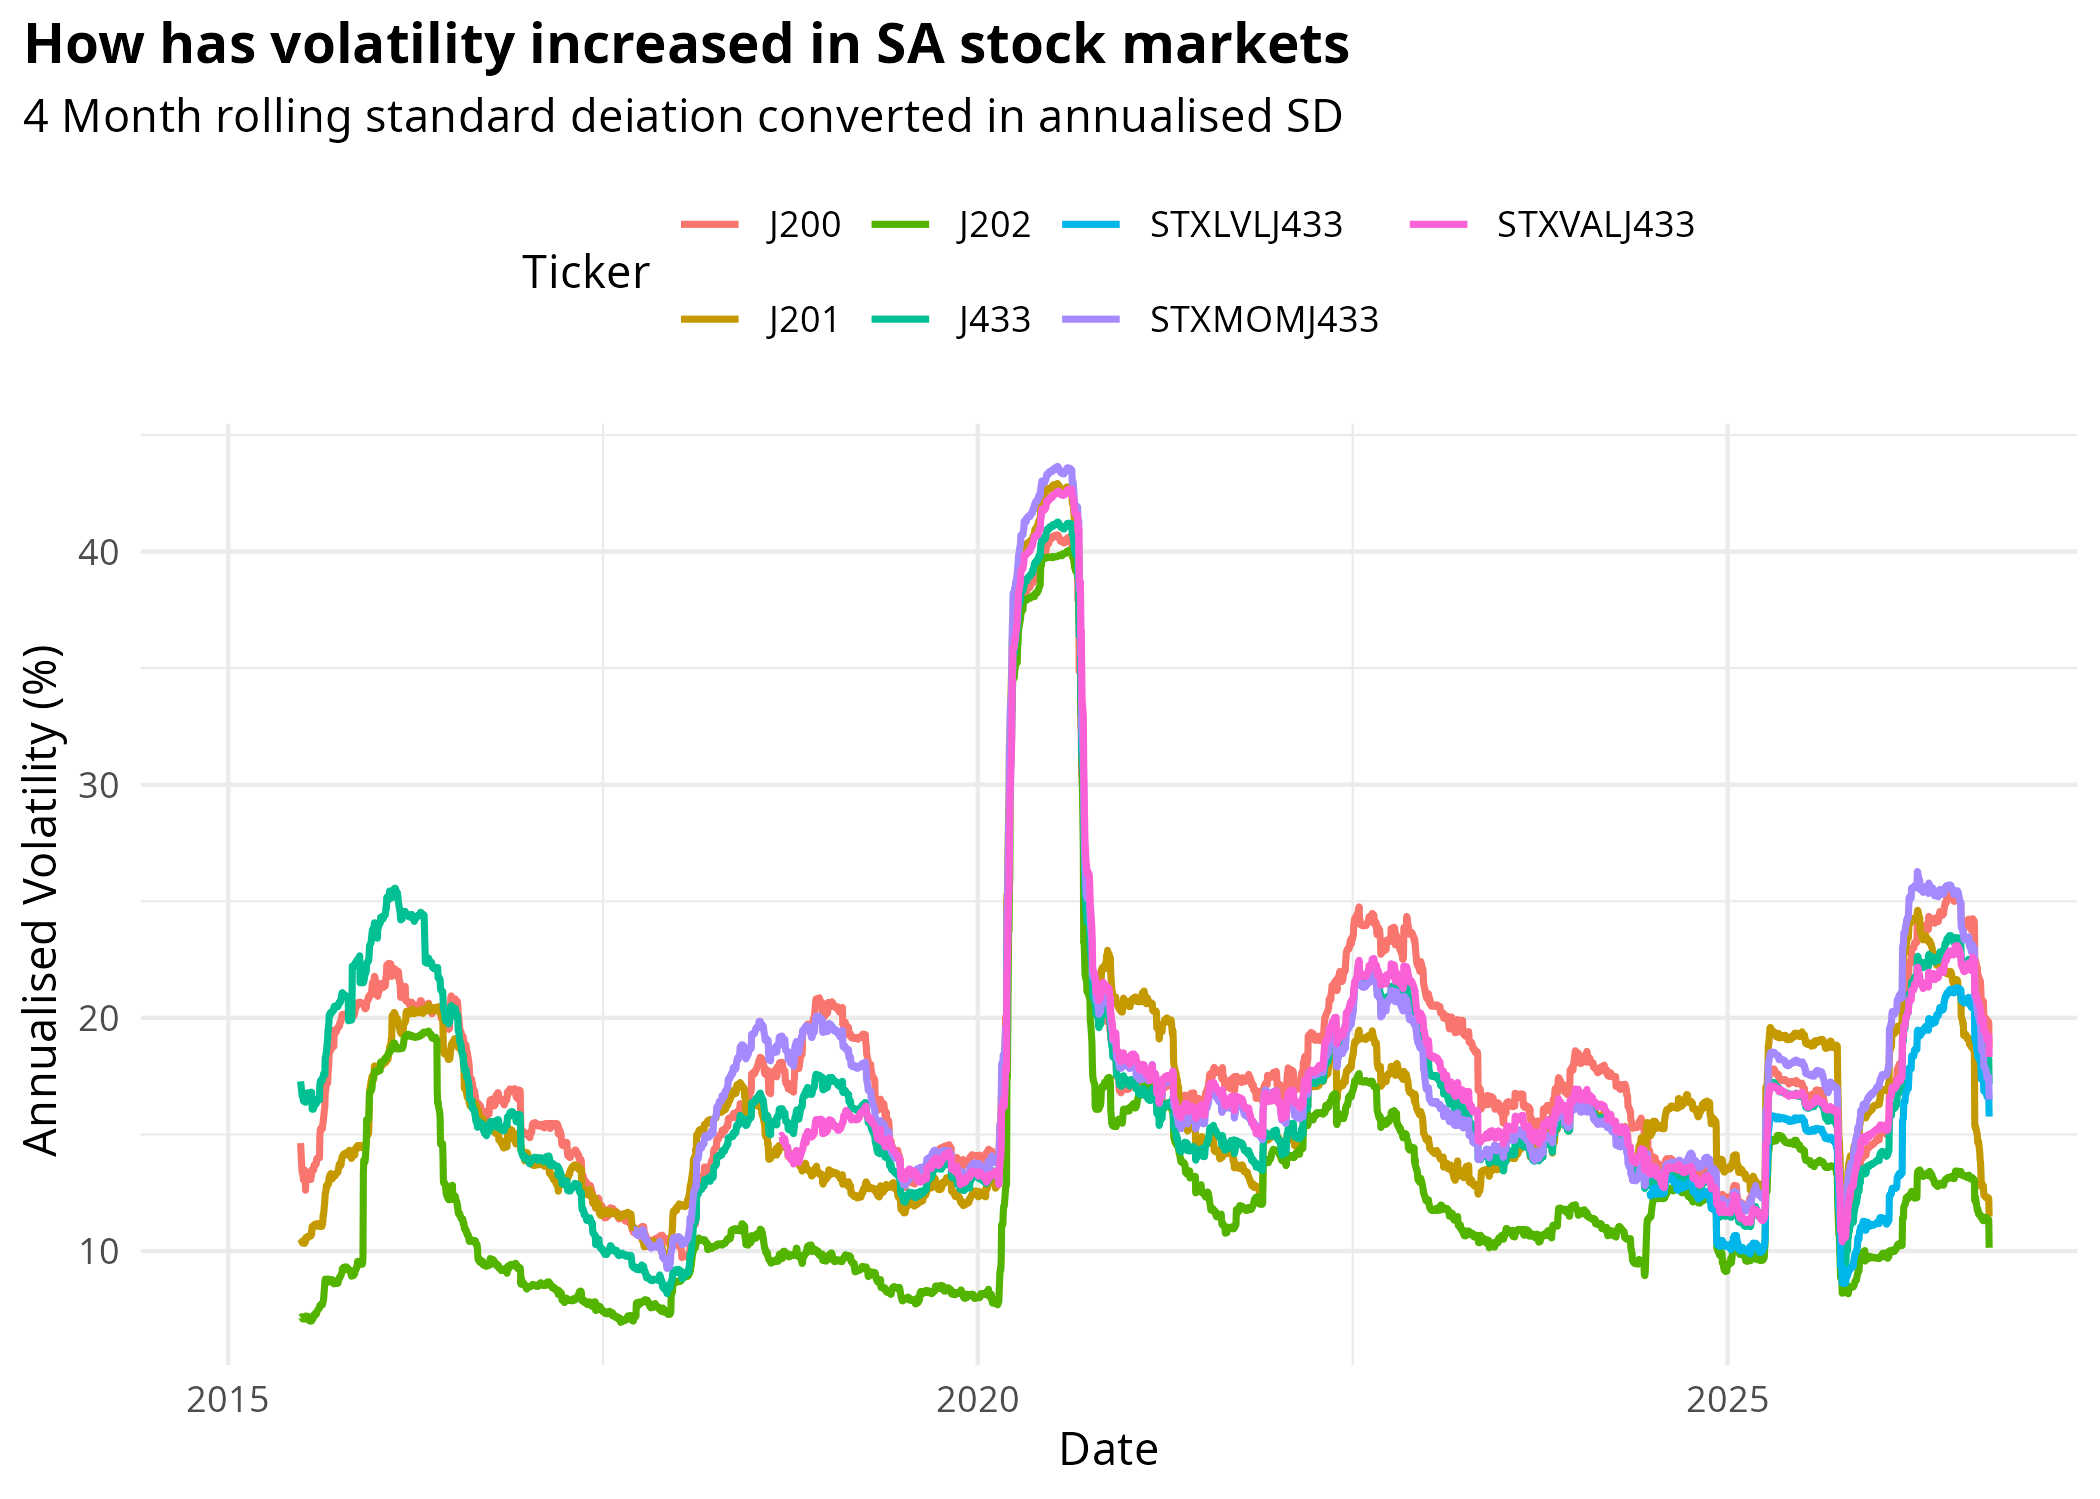
\includegraphics[width=1\linewidth]{figures/rolling_sd_plot}

\subsection{Spillovers (DCC-GARCH)}\label{spillovers-dcc-garch}

\begin{itemize}
\tightlist
\item
  Correlations between the Capped SWIX and the MSCI indices are positive
  and fairly stable. They are highest for Europe (about 0.6) and lowest
  for Japan (about 0.2--0.3).
\item
  Correlations rise in stress, most clearly in COVID (Europe about 0.8,
  the others 0.4--0.6), with smaller rises around 2025--26.
\item
  There is no clear long-run upward trend, so the rises are temporary.
\item
  Diversification across markets therefore weakens when it is needed
  most.
\end{itemize}

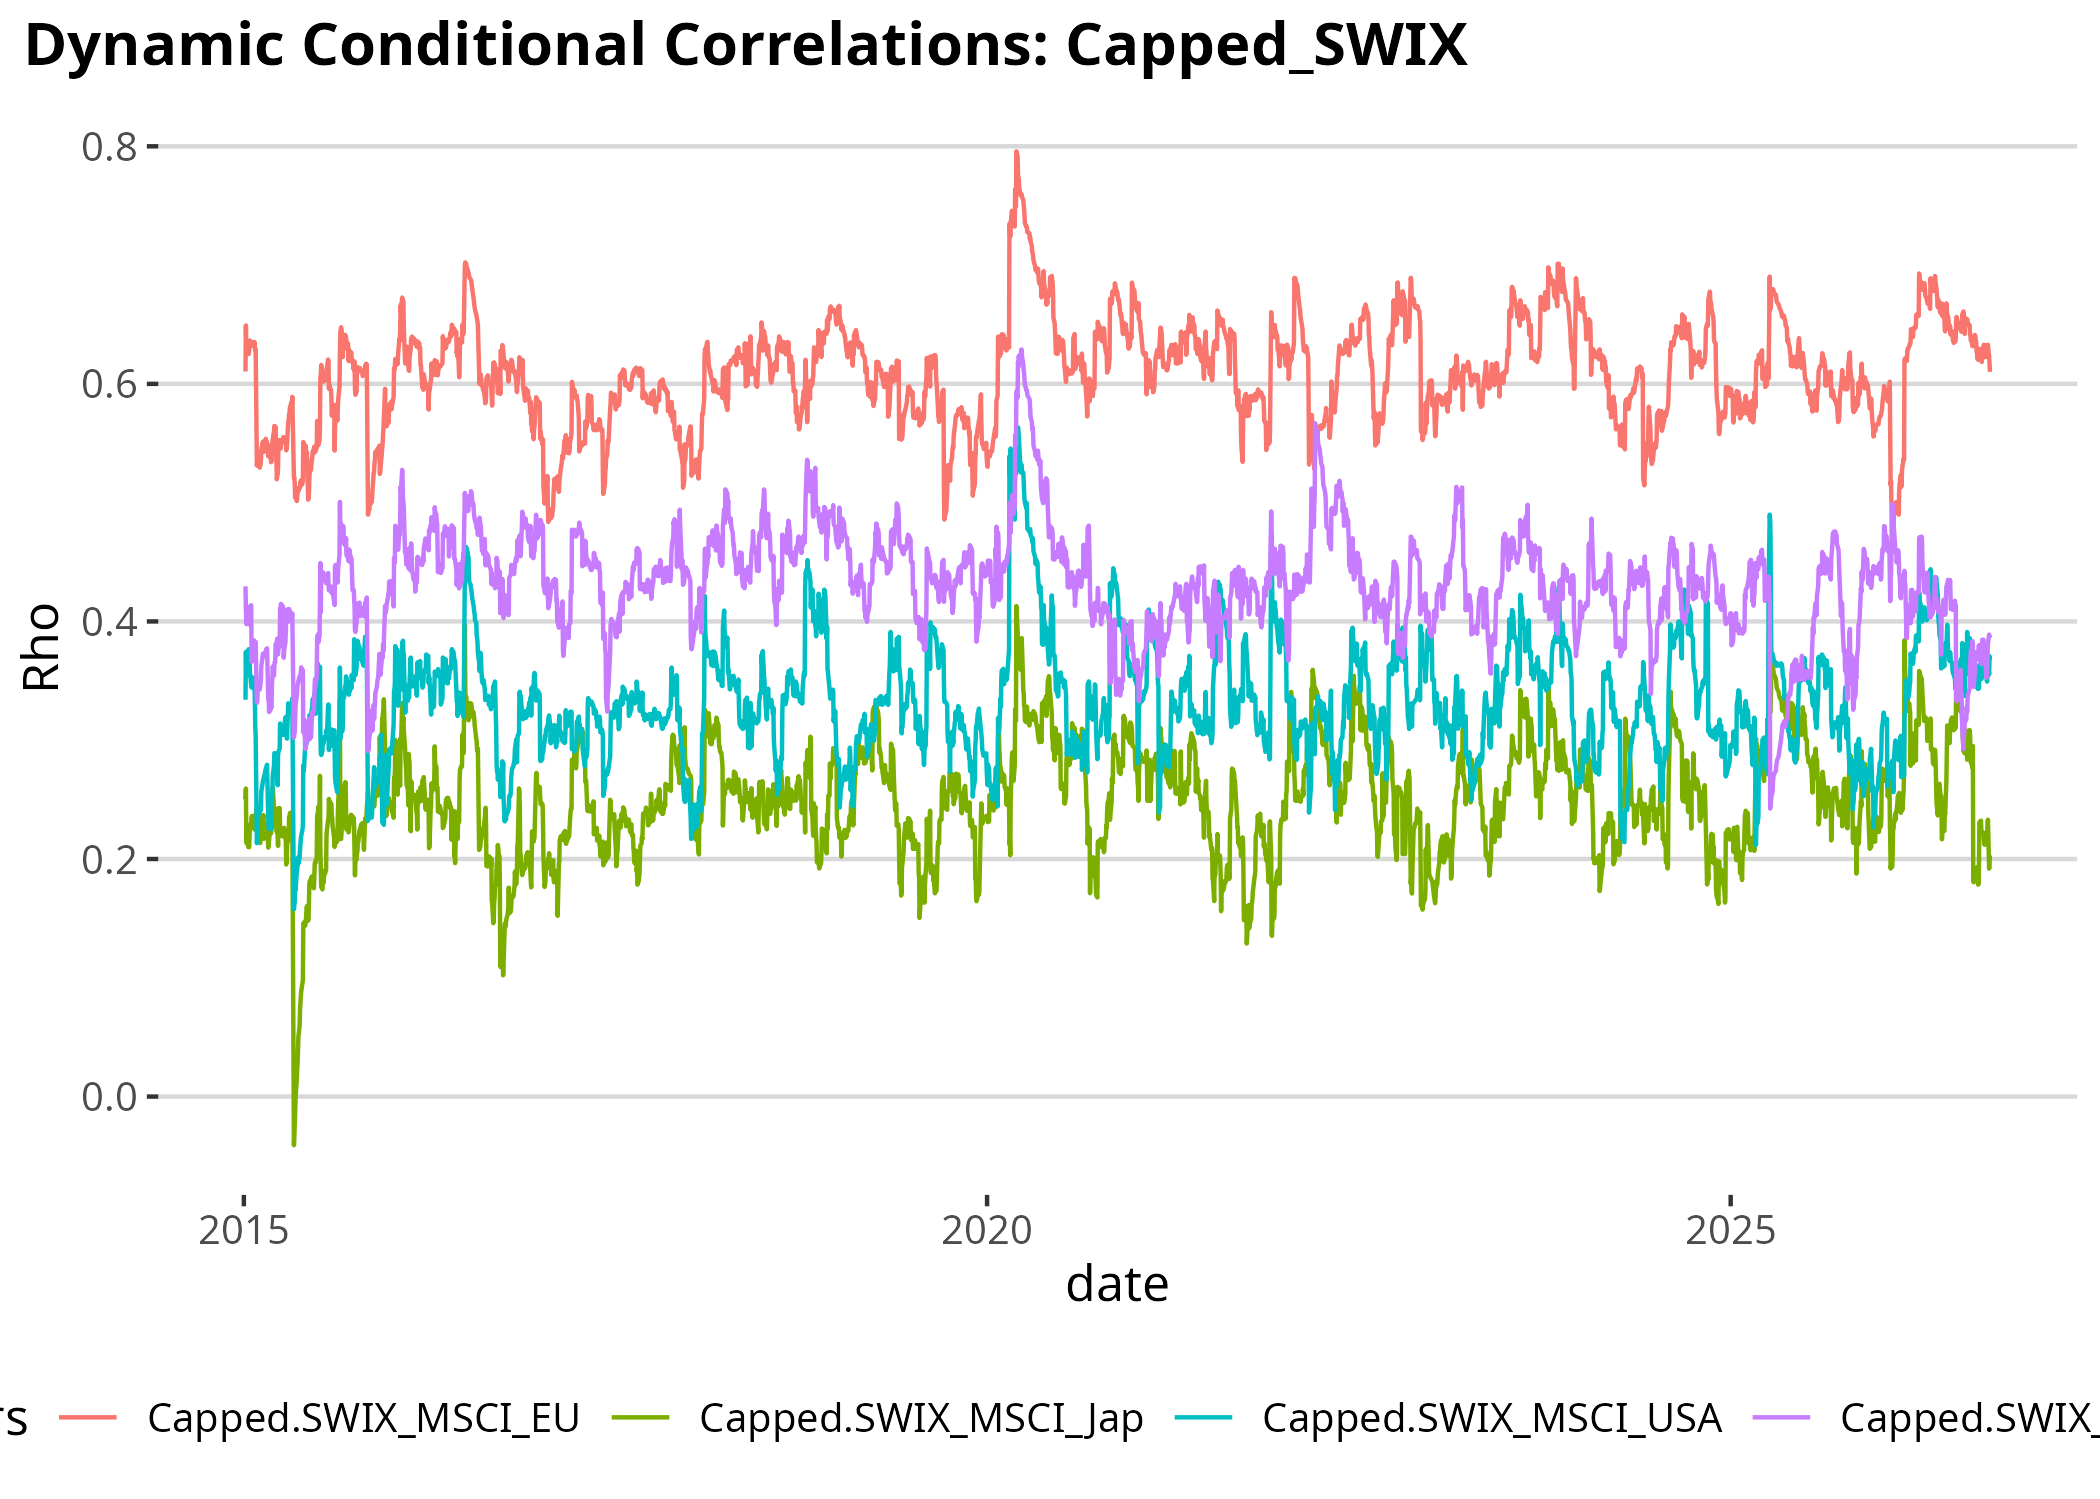
\includegraphics[width=1\linewidth]{figures/g1}

\subsection{Implication for SafeCore}\label{implication-for-safecore}

Volatility is spiky, and the main stress episodes (2020 and 2025--26)
are the real test of how SafeCore handles it. Part B examines this.

\section{Part B}\label{part-b}

\section{Did SafeCore navigate volatility
well?}\label{did-safecore-navigate-volatility-well}

\textbf{Table 1: SafeCore vs Capped SWIX, 2015-01-02 to 2026-09-30
(daily data, annualised with 252 days)}

{\def\LTcaptype{none} % do not increment counter
\begin{longtable}[]{@{}lrr@{}}
\toprule\noalign{}
Metric & SafeCore & Capped SWIX \\
\midrule\noalign{}
\endhead
\bottomrule\noalign{}
\endlastfoot
Annualised return (\%) & 10.75 & 8.65 \\
Annualised volatility (\%) & 17.84 & 17.84 \\
Return / volatility & 0.60 & 0.49 \\
Skewness & -0.41 & -0.44 \\
Excess kurtosis & 4.94 & 6.72 \\
Max drawdown (\%) & -38.99 & -41.66 \\
Downside deviation (\%, ann.) & 12.56 & 12.65 \\
Worst day (\%) & -8.67 & -9.17 \\
Positive days (\%) & 52.13 & 52.06 \\
Beta to Capped SWIX & 0.95 & \\
Tracking error (\%, ann.) & 5.66 & \\
Information ratio & 0.37 & \\
Up capture (\%) & 99.13 & \\
Down capture (\%) & 97.04 & \\
\end{longtable}
}

\begin{itemize}
\tightlist
\item
  \textbf{No volatility reduction.} Both volatilities are 17.84\% and
  beta is 0.95. This is expected, since volatility is not an input to
  SafeCore's construction.
\item
  \textbf{Better return per unit of risk.} SafeCore earned about 2.1
  percentage points more per year, lifting return/volatility from 0.49
  to 0.60.
\item
  \textbf{Slightly better tail outcomes.} Max drawdown was 39.0\%
  against 41.7\%, the worst day was milder and excess kurtosis was lower
  (4.94 vs 6.72). Downside deviation is almost identical.
\item
  \textbf{Little protection.} Capture ratios of 99\% (up) and 97\%
  (down) show the fund moves almost one-for-one with the benchmark. The
  3-point downside advantage is small.
\item
  \textbf{Weak evidence of skill.} An information ratio of 0.37 over
  about 11.75 years implies a t-statistic of roughly 1.3, so the
  outperformance is not statistically convincing.
\end{itemize}

\textbf{Table 2: Average monthly return (\%) by volatility regime}

{\def\LTcaptype{none} % do not increment counter
\begin{longtable}[]{@{}
  >{\raggedright\arraybackslash}p{(\linewidth - 8\tabcolsep) * \real{0.4557}}
  >{\raggedleft\arraybackslash}p{(\linewidth - 8\tabcolsep) * \real{0.1013}}
  >{\raggedleft\arraybackslash}p{(\linewidth - 8\tabcolsep) * \real{0.1266}}
  >{\raggedleft\arraybackslash}p{(\linewidth - 8\tabcolsep) * \real{0.1646}}
  >{\raggedleft\arraybackslash}p{(\linewidth - 8\tabcolsep) * \real{0.1519}}@{}}
\toprule\noalign{}
\begin{minipage}[b]{\linewidth}\raggedright
Regime
\end{minipage} & \begin{minipage}[b]{\linewidth}\raggedleft
Months
\end{minipage} & \begin{minipage}[b]{\linewidth}\raggedleft
SafeCore
\end{minipage} & \begin{minipage}[b]{\linewidth}\raggedleft
Capped SWIX
\end{minipage} & \begin{minipage}[b]{\linewidth}\raggedleft
Difference
\end{minipage} \\
\midrule\noalign{}
\endhead
\bottomrule\noalign{}
\endlastfoot
High global vol (top quartile VIX) & 36 & 0.93 & 0.84 & 0.08 \\
Other months & 105 & 0.94 & 0.77 & 0.17 \\
\end{longtable}
}

\begin{itemize}
\tightlist
\item
  SafeCore's advantage over the benchmark is smaller in high-volatility
  months (+0.08 vs +0.17 percentage points per month). That is the
  opposite of protection, although both gaps are small.
\item
  \textbf{Verdict:} SafeCore tracked the market's volatility rather than
  navigating it, with modest outperformance and a slightly shallower
  drawdown.
\end{itemize}

\subsection{. Where does the volatility come
from?}\label{where-does-the-volatility-come-from}

\paragraph{Stocks and sectors (latest rebalance, 250-day
covariance)}\label{stocks-and-sectors-latest-rebalance-250-day-covariance}

\textbf{Table 3: Top 10 stocks by contribution to portfolio variance}

{\def\LTcaptype{none} % do not increment counter
\begin{longtable}[]{@{}
  >{\raggedright\arraybackslash}p{(\linewidth - 8\tabcolsep) * \real{0.0921}}
  >{\raggedright\arraybackslash}p{(\linewidth - 8\tabcolsep) * \real{0.1974}}
  >{\raggedleft\arraybackslash}p{(\linewidth - 8\tabcolsep) * \real{0.1579}}
  >{\raggedleft\arraybackslash}p{(\linewidth - 8\tabcolsep) * \real{0.3026}}
  >{\raggedleft\arraybackslash}p{(\linewidth - 8\tabcolsep) * \real{0.2500}}@{}}
\toprule\noalign{}
\begin{minipage}[b]{\linewidth}\raggedright
Stock
\end{minipage} & \begin{minipage}[b]{\linewidth}\raggedright
Sector
\end{minipage} & \begin{minipage}[b]{\linewidth}\raggedleft
Weight (\%)
\end{minipage} & \begin{minipage}[b]{\linewidth}\raggedleft
Risk contribution (\%)
\end{minipage} & \begin{minipage}[b]{\linewidth}\raggedleft
Beta to portfolio
\end{minipage} \\
\midrule\noalign{}
\endhead
\bottomrule\noalign{}
\endlastfoot
ANG & Resources & 11.97 & 27.76 & 2.32 \\
GFI & Resources & 7.48 & 17.25 & 2.31 \\
VAL & Unclassified* & 4.42 & 10.41 & 2.36 \\
MTN & Industrials & 8.80 & 6.30 & 0.72 \\
SBK & Financials & 10.13 & 6.18 & 0.61 \\
PAN & Unclassified* & 2.75 & 5.74 & 2.09 \\
ABG & Financials & 7.23 & 4.12 & 0.57 \\
BHG & Resources & 4.69 & 3.53 & 0.75 \\
FSR & Financials & 5.15 & 3.14 & 0.61 \\
SSW & Resources & 0.99 & 2.44 & 2.47 \\
\end{longtable}
}

*Sector missing in the data. VAL and PAN are precious-metals miners.

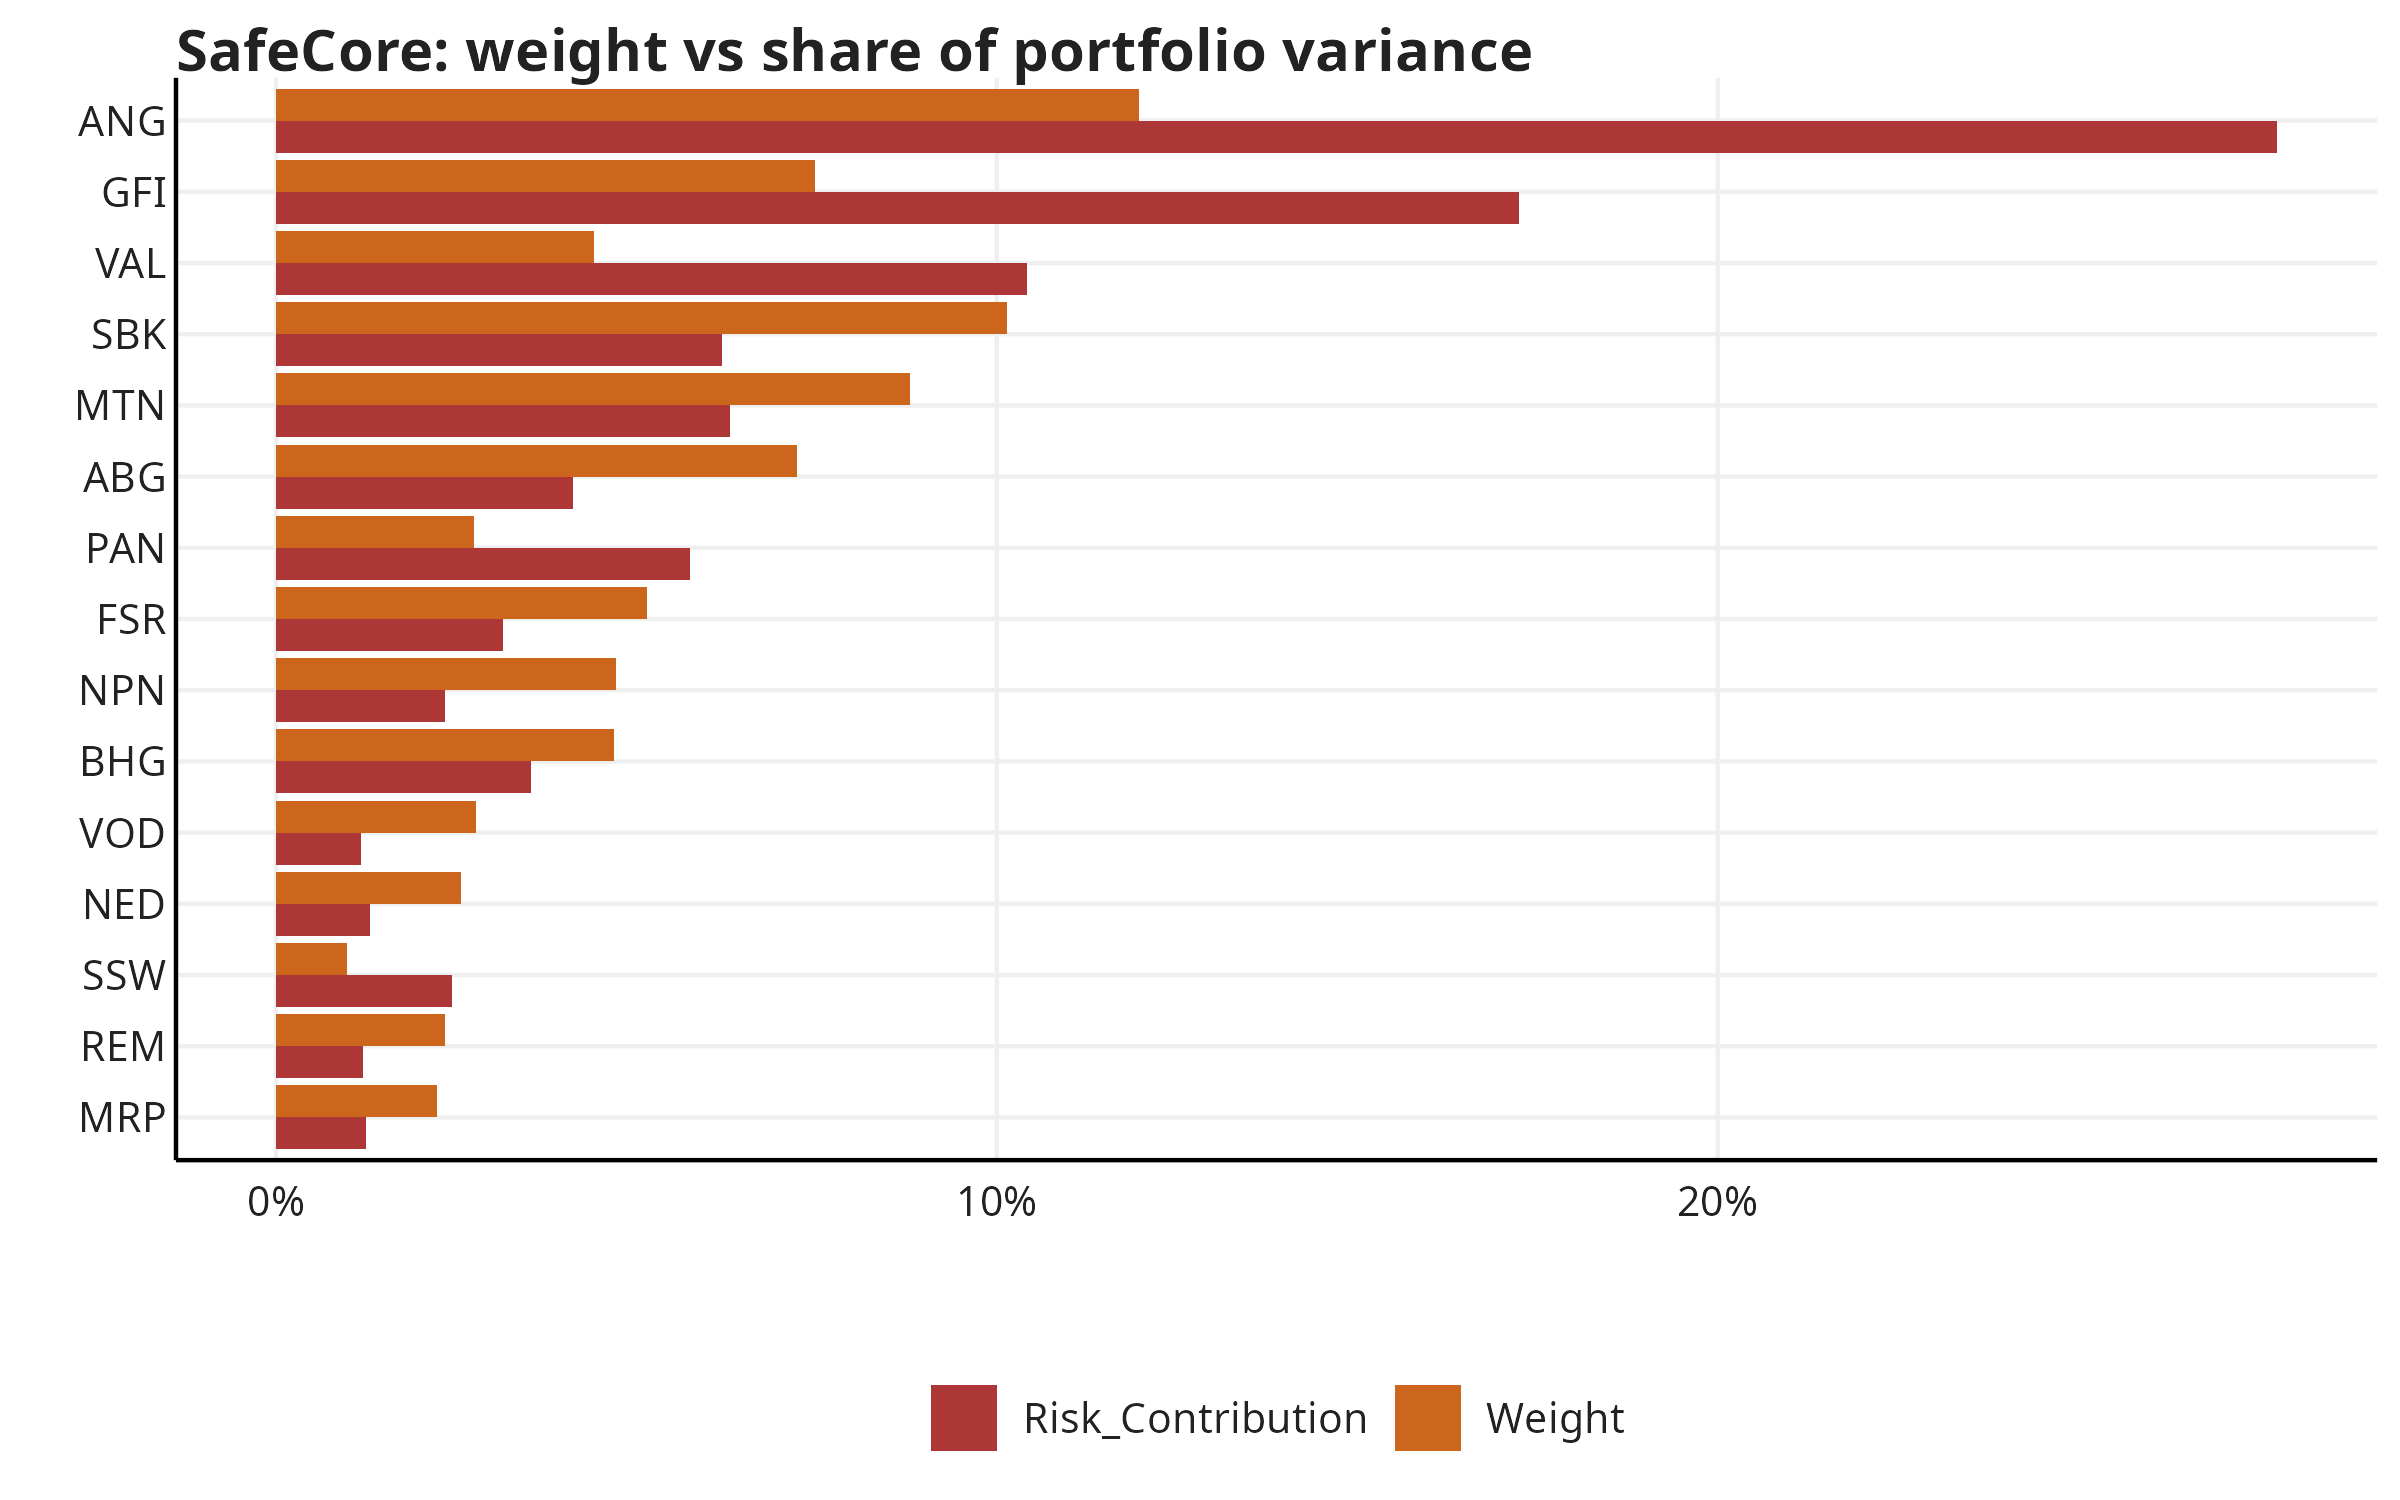
\includegraphics[width=1\linewidth]{figures/top15rc}

\begin{itemize}
\tightlist
\item
  \textbf{Risk is far more concentrated than weights.} Five gold and
  platinum miners (ANG, GFI, VAL, PAN, SSW) are 27.6\% of the fund by
  weight but 63.6\% of its variance.
\item
  Their betas to the portfolio are 2.1 to 2.5, so each 1\% of weight
  carries about 2.3\% of portfolio variance.
\item
  Financials and industrials are the opposite. SBK, ABG, FSR and MTN
  have betas of 0.6 to 0.75 and contribute less risk than their weights.
\end{itemize}

\textbf{Table 4: Sector contribution to portfolio variance}

{\def\LTcaptype{none} % do not increment counter
\begin{longtable}[]{@{}lrrr@{}}
\toprule\noalign{}
Sector & Weight (\%) & Risk contribution (\%) & Risk / weight \\
\midrule\noalign{}
\endhead
\bottomrule\noalign{}
\endlastfoot
Resources & 32.98 & 52.01 & 1.58 \\
Financials & 31.34 & 17.73 & 0.57 \\
Unclassified* & 7.17 & 16.15 & 2.25 \\
Industrials & 25.98 & 13.25 & 0.51 \\
Property & 2.53 & 0.86 & 0.34 \\
\end{longtable}
}

\begin{itemize}
\tightlist
\item
  Resources are 33\% of weight but 52\% of risk. Counting the two
  unclassified miners as Resources gives 40\% of weight and 68\% of
  risk.
\end{itemize}

\subsubsection{Statistical factors (PCA)}\label{statistical-factors-pca}

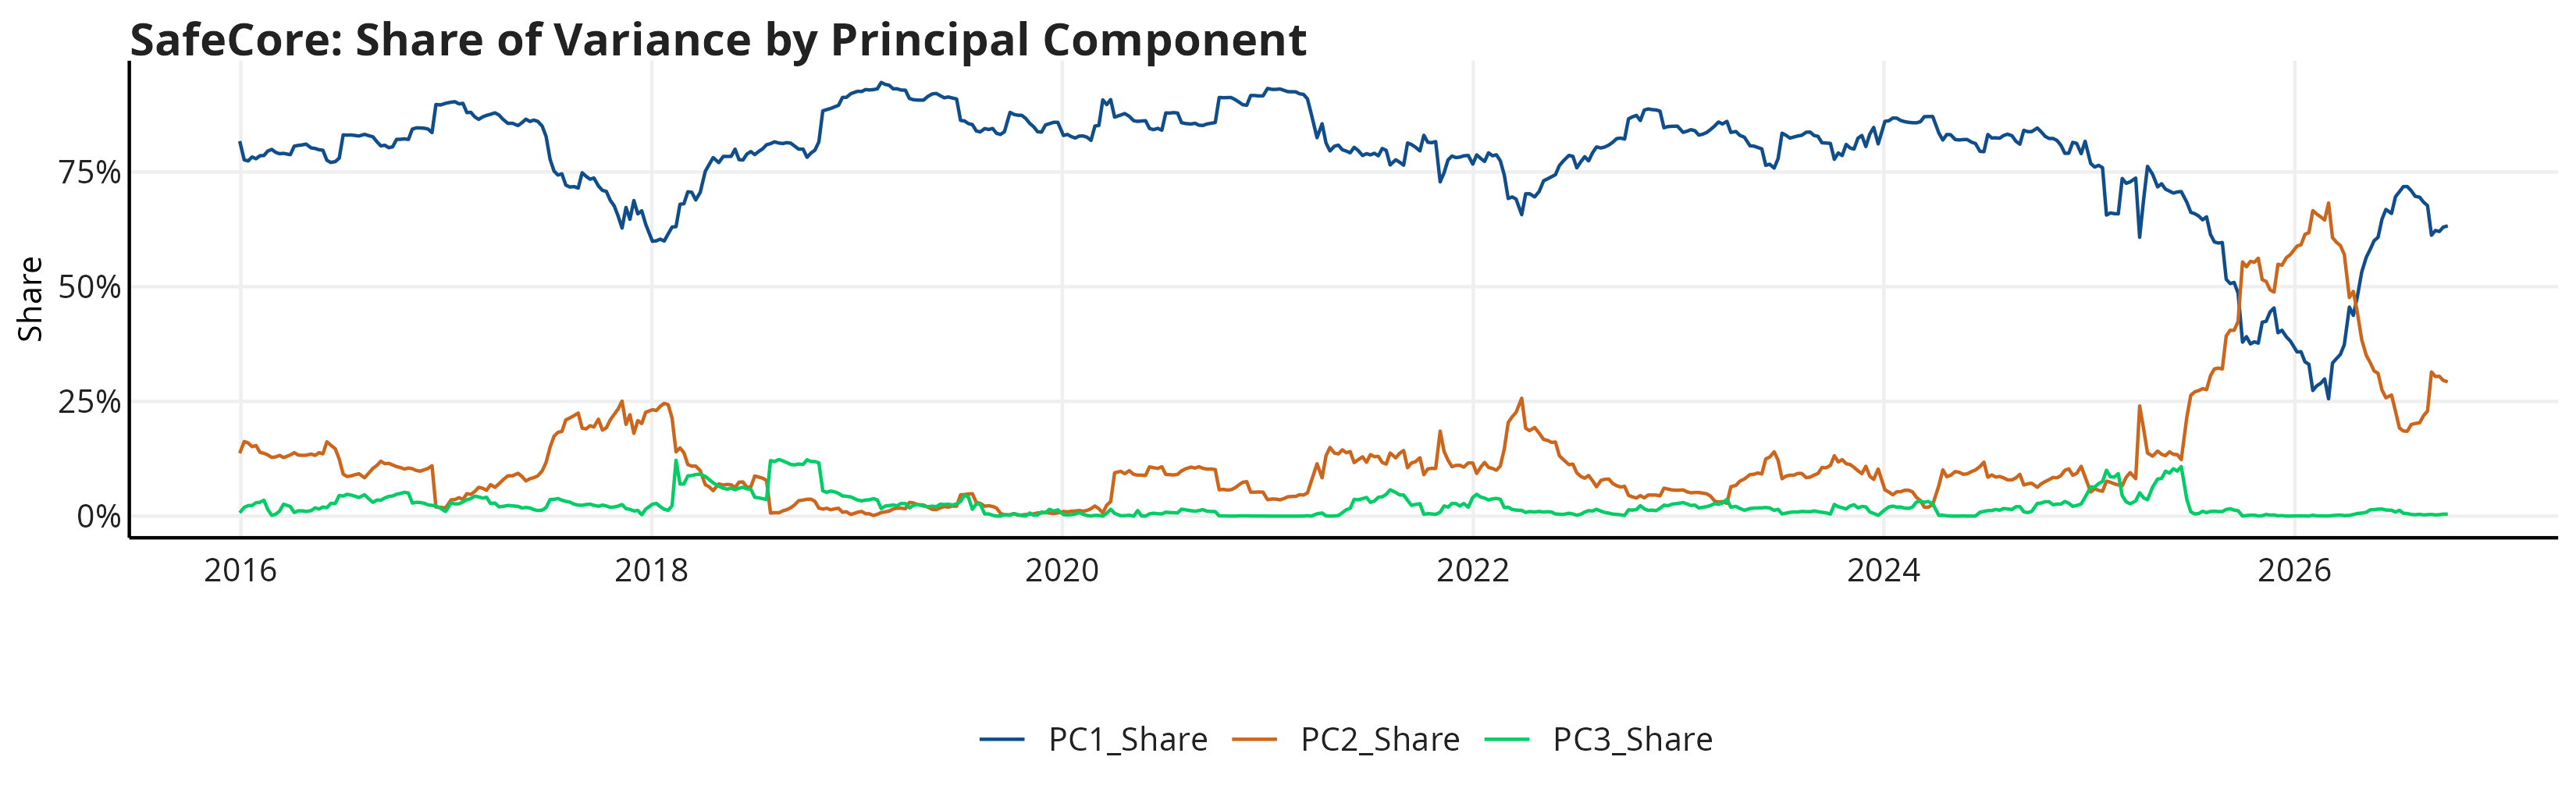
\includegraphics[width=1\linewidth]{figures/prop_var}

\begin{itemize}
\tightlist
\item
  At the latest rebalance, PC1 accounts for about 88\% of portfolio
  variance and PC3 about 7\%. Every other component is 2\% or less.
\end{itemize}

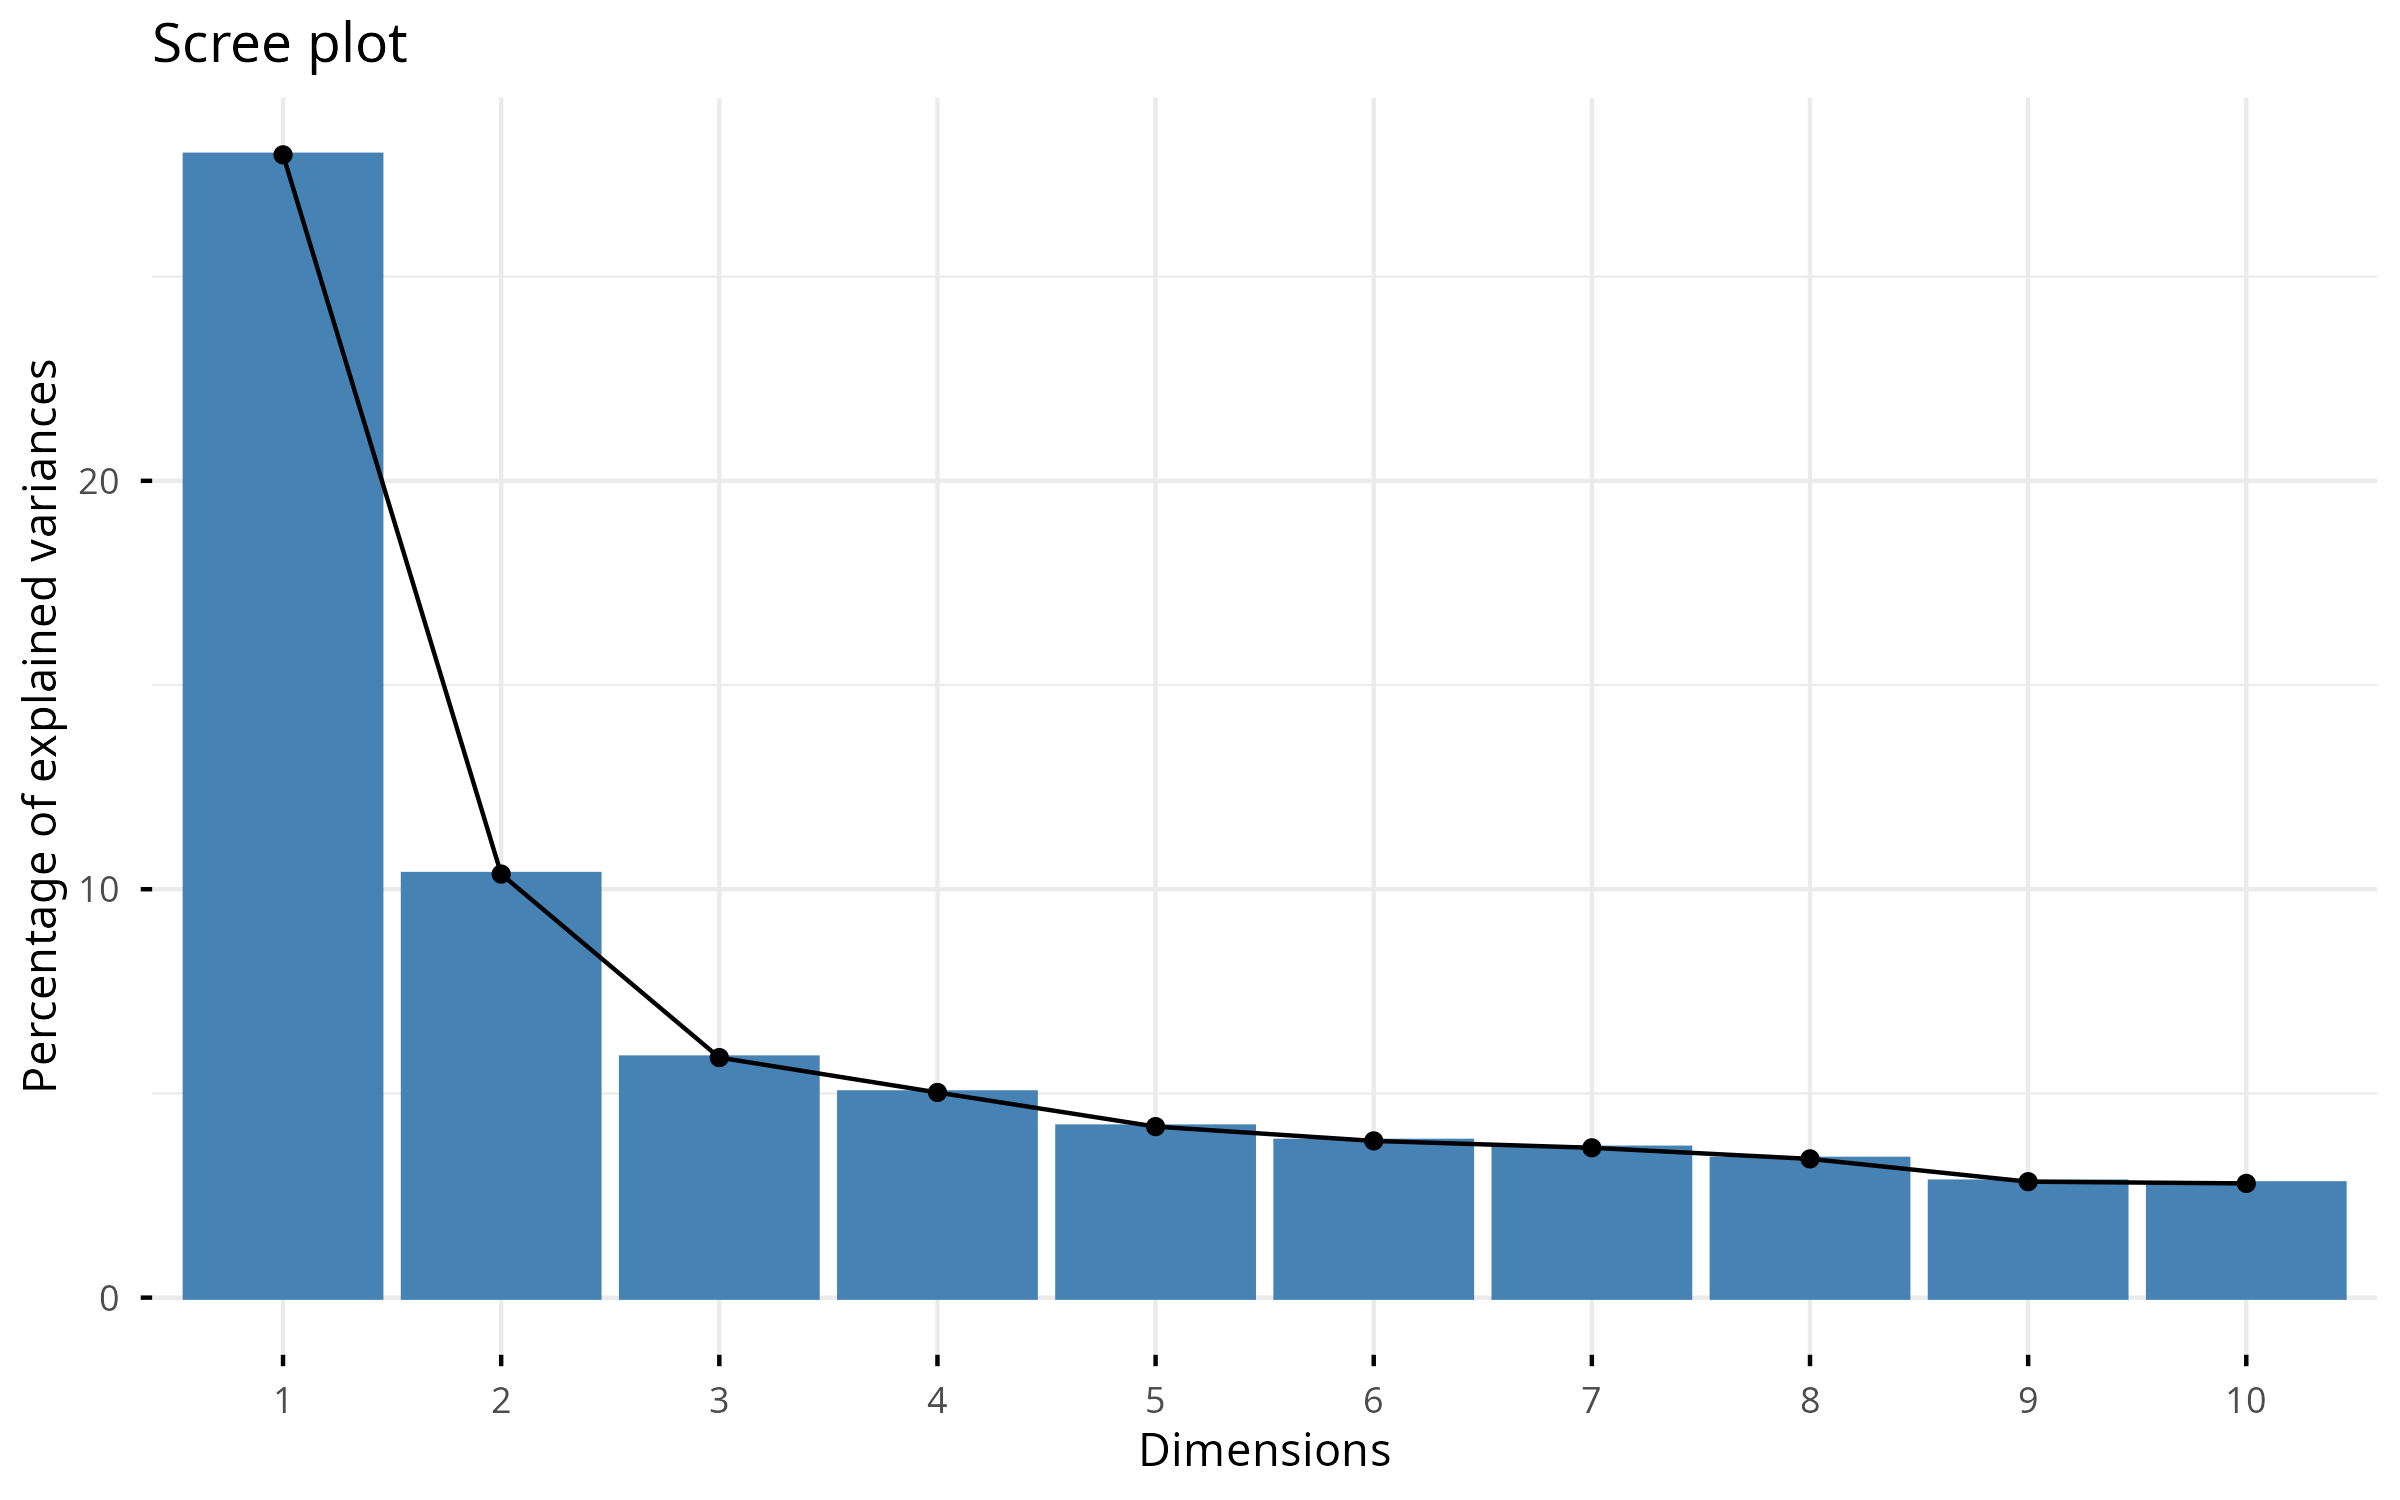
\includegraphics[width=1\linewidth]{figures/screeplot}

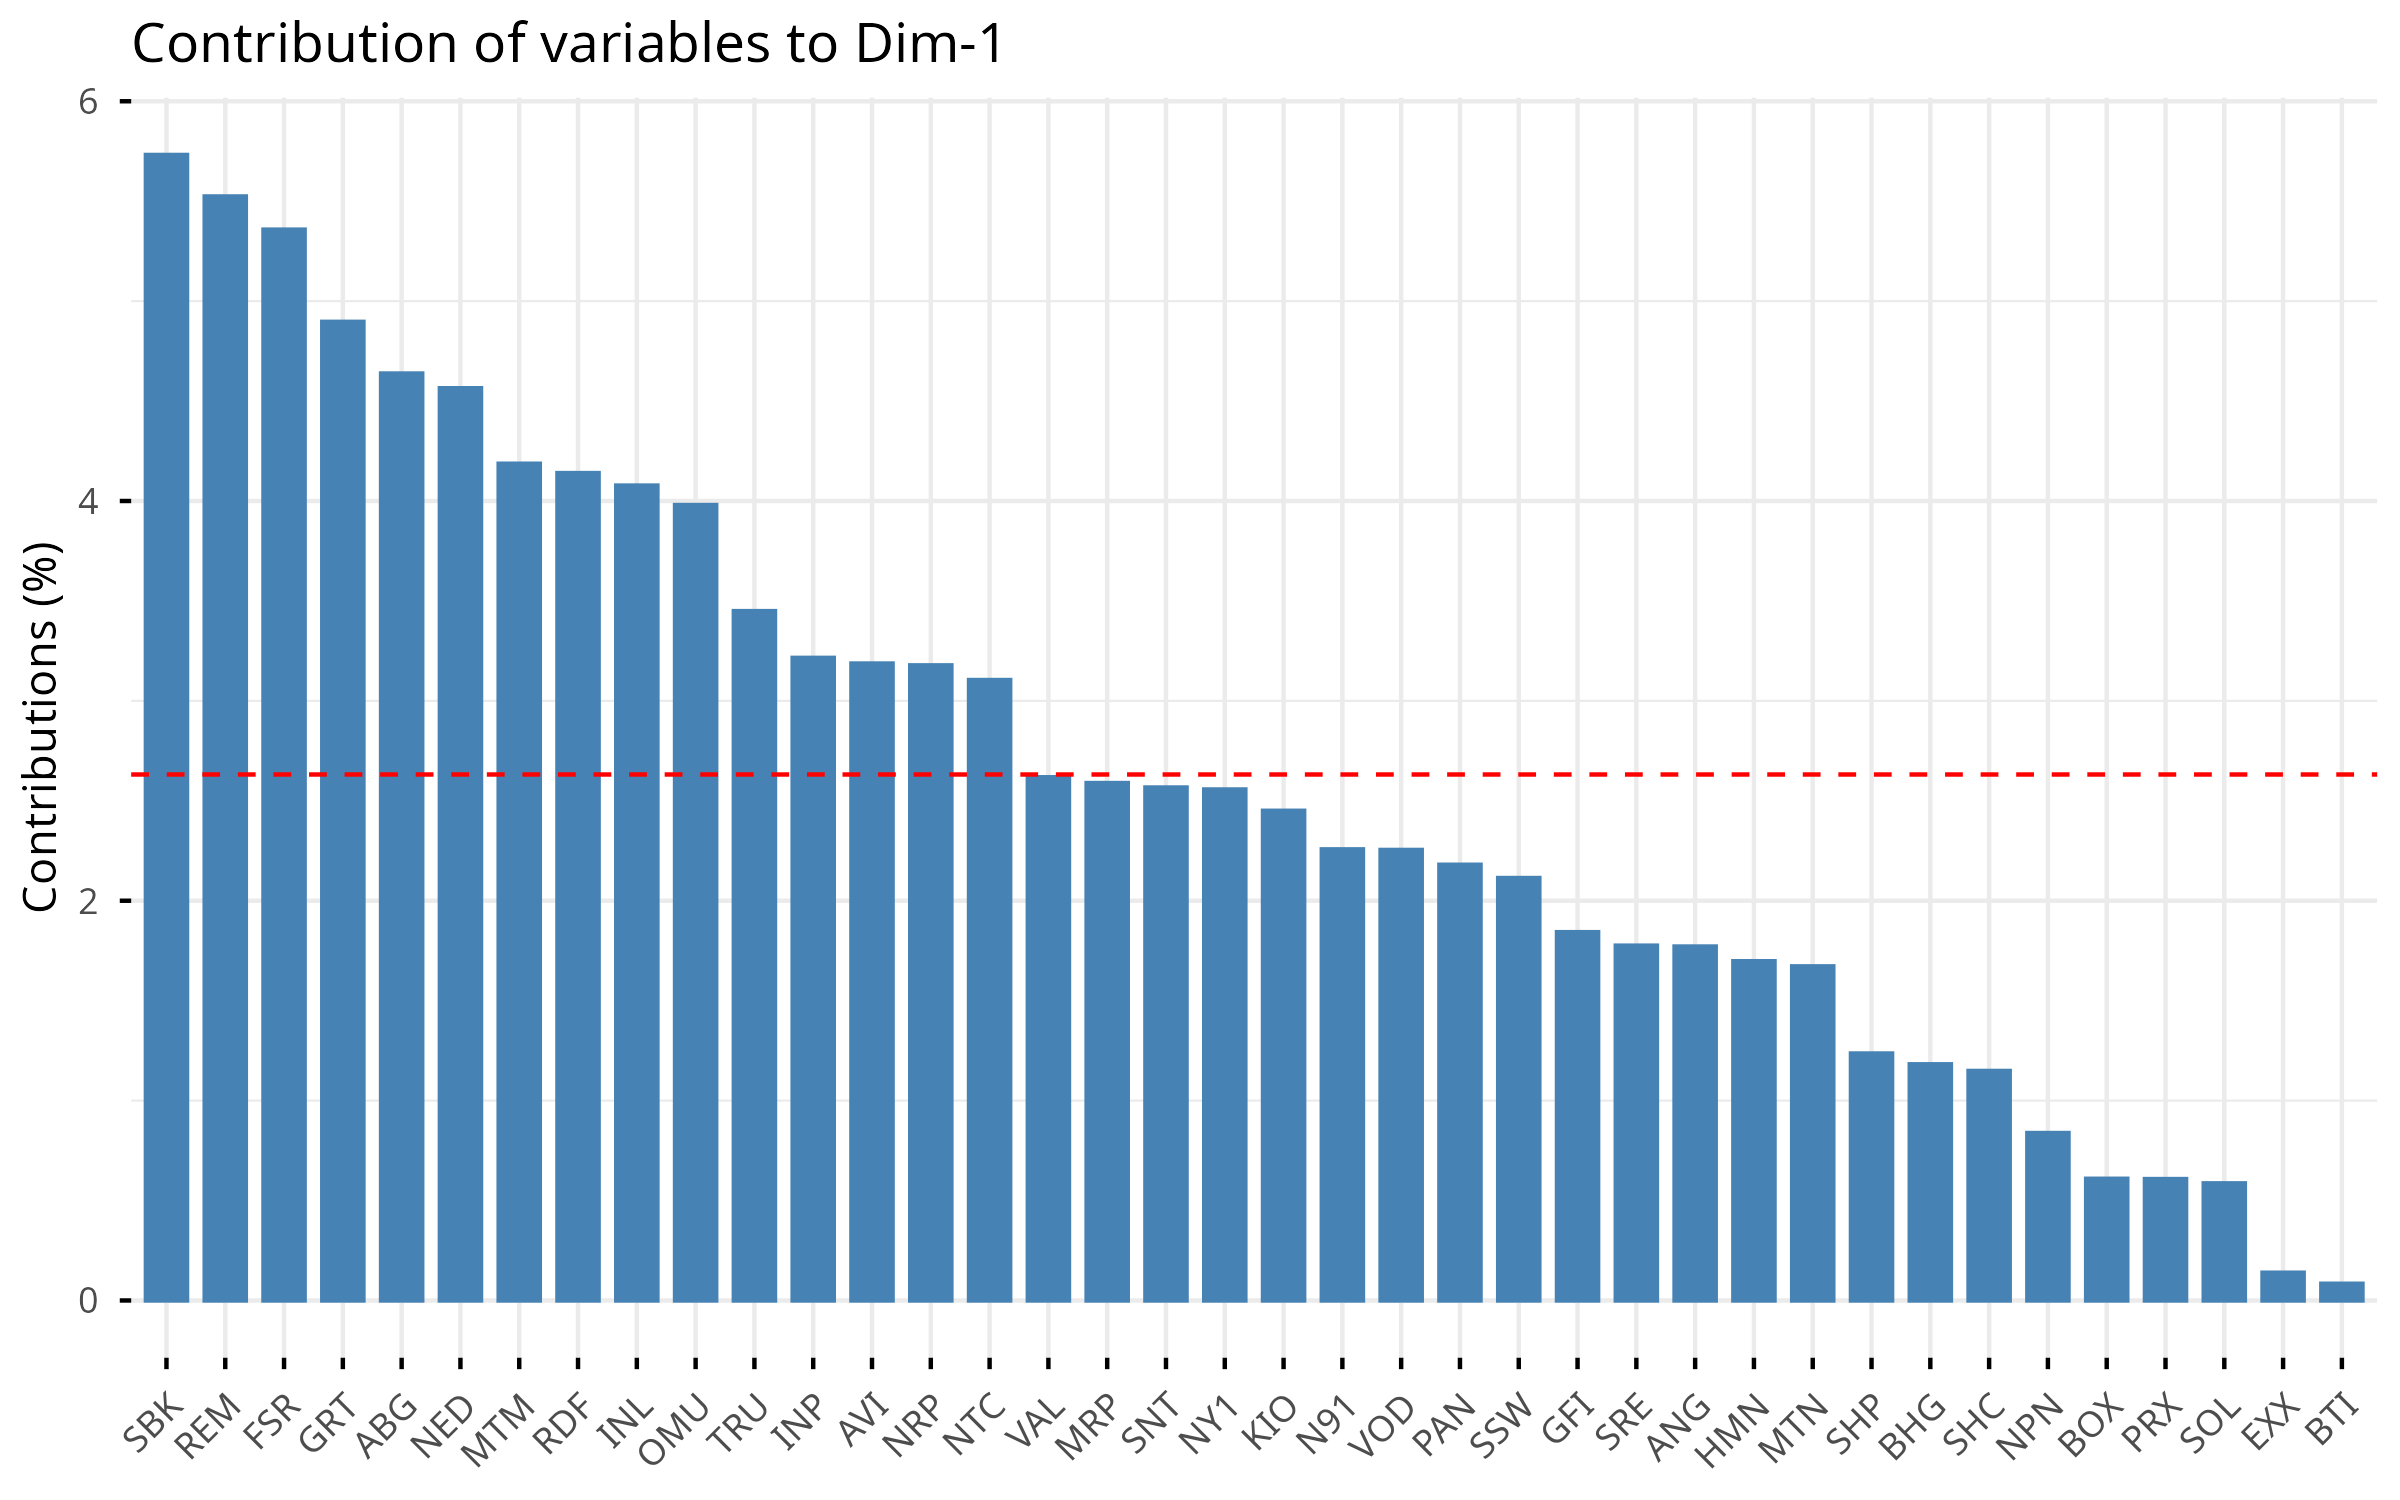
\includegraphics[width=1\linewidth]{figures/stock_contrib}

\begin{itemize}
\tightlist
\item
  Across the stock universe, PC1 explains about 28\% of variance and PC2
  about 10.4\%.
\item
  PC1 is a broad domestic factor, led by financials and property (SBK,
  REM, FSR, GRT, ABG, NED).
\item
  PC2 is the precious-metals factor (ANG, GFI, SSW, PAN, VAL). SOL and
  BTI point away from the main cluster, which marks them as
  diversifiers.
\item
  The portfolio arrow lies between PC1 and PC2, so SafeCore is exposed
  to both the market and the metals factor.
\item
  The portfolio's PC1 share (61\%) is higher than the scree plot's 28\%
  because the portfolio is a weighted average, so stock-specific noise
  cancels and the common factors dominate.
\end{itemize}

\subsubsection{Through time}\label{through-time}

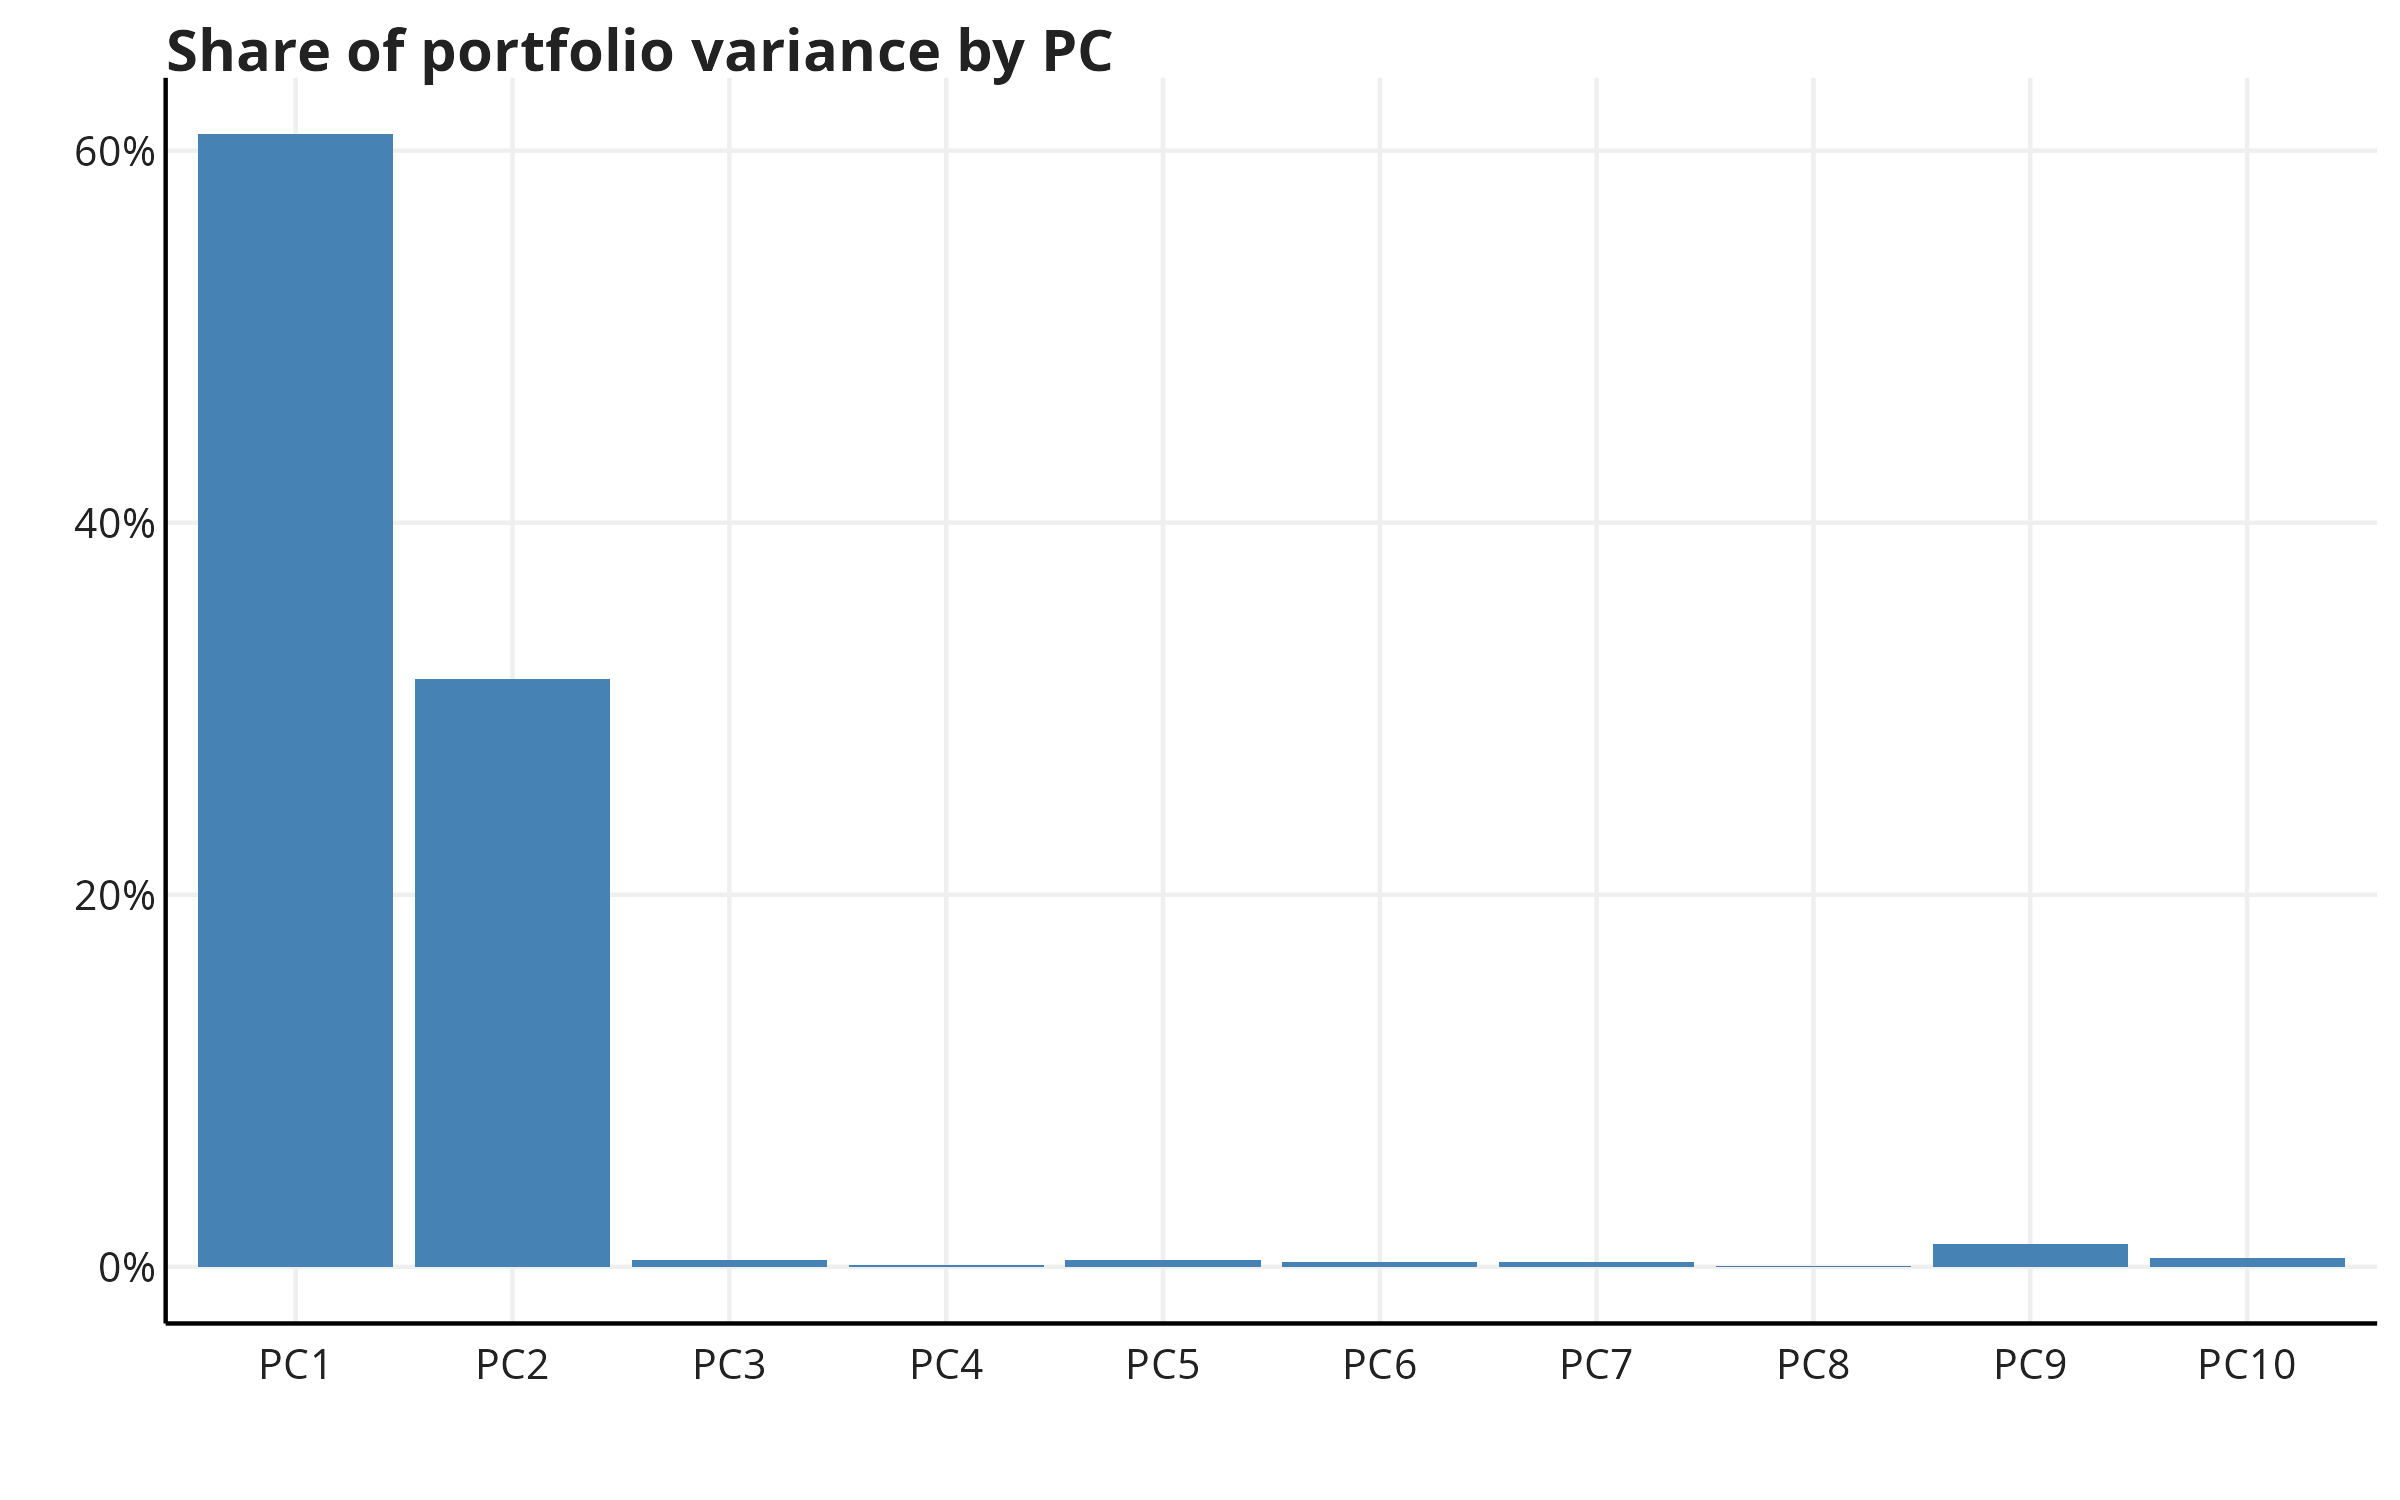
\includegraphics[width=1\linewidth]{figures/share_port_var_pc}

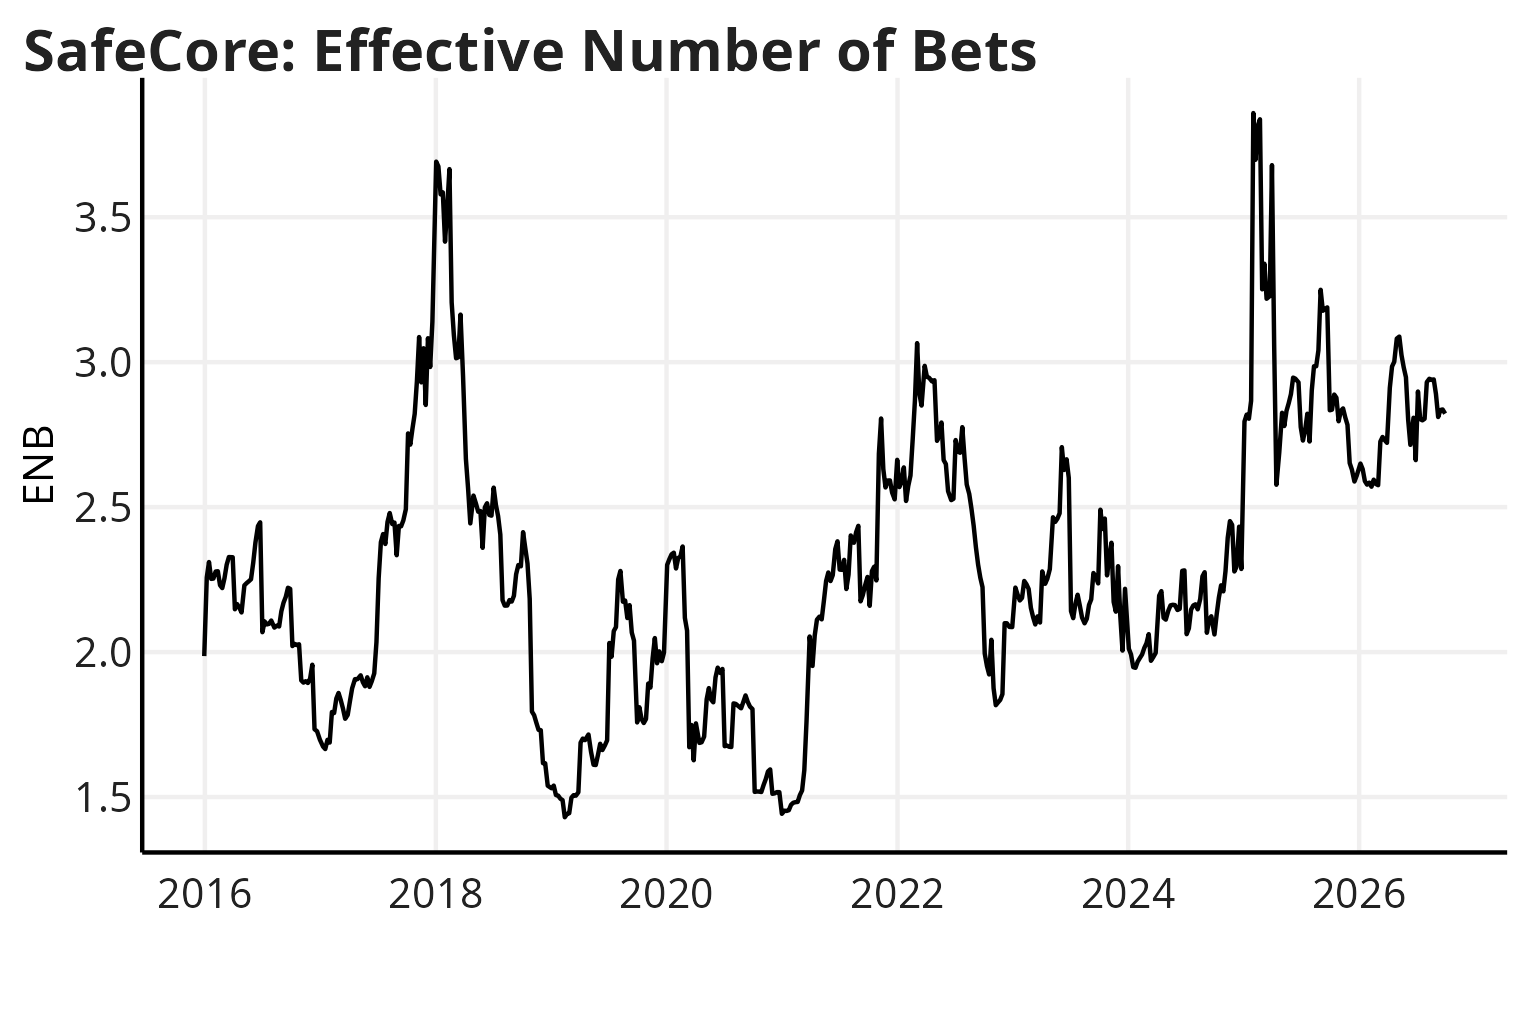
\includegraphics[width=1\linewidth]{figures/SafeCore_eff_num_bets}

\begin{itemize}
\tightlist
\item
  From 2016 to 2024, PC1 explains most of SafeCore's variance (about
  75\% to 93\%), with dips to about 60\% to 65\% in 2018 and 2022.
\item
  In 2025 and 2026 the picture changes: PC2 rises to about 55\% to 68\%
  around late 2025 to early 2026, while PC1 falls to about 26\%. By the
  end of the sample the split is about 63\% and 30\%.
\item
  ENB mostly sits between 1.5 and 2.5, with troughs in early 2019 and
  early 2021 (about 1.45) and peaks in early 2018 (about 3.7) and early
  2025 (about 3.85).
\item
  Since 2025, ENB has been higher (about 2.6 to 3.3). This is because
  the precious-metals factor has become a second major source of risk,
  not because risk has fallen.
\item
  COVID is not a special episode in the ENB series, so there is no
  evidence that concentration changes in a stress period in general.
\end{itemize}

\subsection{Diversifiers and
concentrators}\label{diversifiers-and-concentrators}

A stock's risk contribution divided by its weight equals its beta to the
portfolio. A beta below 1 means it reduces concentration relative to its
size. Positions under 0.5\% are excluded.

\textbf{Table 5: Lowest and highest portfolio betas}

{\def\LTcaptype{none} % do not increment counter
\begin{longtable}[]{@{}
  >{\raggedright\arraybackslash}p{(\linewidth - 10\tabcolsep) * \real{0.1591}}
  >{\raggedright\arraybackslash}p{(\linewidth - 10\tabcolsep) * \real{0.0795}}
  >{\raggedright\arraybackslash}p{(\linewidth - 10\tabcolsep) * \real{0.1477}}
  >{\raggedleft\arraybackslash}p{(\linewidth - 10\tabcolsep) * \real{0.1364}}
  >{\raggedleft\arraybackslash}p{(\linewidth - 10\tabcolsep) * \real{0.2614}}
  >{\raggedleft\arraybackslash}p{(\linewidth - 10\tabcolsep) * \real{0.2159}}@{}}
\toprule\noalign{}
\begin{minipage}[b]{\linewidth}\raggedright
Type
\end{minipage} & \begin{minipage}[b]{\linewidth}\raggedright
Stock
\end{minipage} & \begin{minipage}[b]{\linewidth}\raggedright
Sector
\end{minipage} & \begin{minipage}[b]{\linewidth}\raggedleft
Weight (\%)
\end{minipage} & \begin{minipage}[b]{\linewidth}\raggedleft
Risk contribution (\%)
\end{minipage} & \begin{minipage}[b]{\linewidth}\raggedleft
Beta to portfolio
\end{minipage} \\
\midrule\noalign{}
\endhead
\bottomrule\noalign{}
\endlastfoot
Diversifier & BTI & Industrials & 0.81 & -0.13 & -0.16 \\
Diversifier & SOL & Resources & 4.84 & -0.52 & -0.11 \\
Diversifier & SHP & Industrials & 2.06 & 0.41 & 0.20 \\
Diversifier & NRP & Property & 1.07 & 0.25 & 0.23 \\
Diversifier & EXX & Resources & 1.68 & 0.44 & 0.26 \\
Diversifier & AVI & Industrials & 0.99 & 0.34 & 0.35 \\
Diversifier & PRX & Industrials & 1.35 & 0.51 & 0.37 \\
Diversifier & INL & Financials & 0.58 & 0.24 & 0.41 \\
Diversifier & VOD & Industrials & 2.78 & 1.17 & 0.42 \\
Diversifier & NTC & Industrials & 0.52 & 0.22 & 0.43 \\
Diversifier & SBK & Financials & 10.13 & 6.18 & 0.61 \\
Diversifier & FSR & Financials & 5.15 & 3.14 & 0.61 \\
Diversifier & MTN & Industrials & 8.80 & 6.30 & 0.72 \\
Diversifier & BHG & Resources & 4.69 & 3.53 & 0.75 \\
Diversifier & KIO & Resources & 1.34 & 1.12 & 0.84 \\
Concentrator & PAN & Unclassified* & 2.75 & 5.74 & 2.09 \\
Concentrator & GFI & Resources & 7.48 & 17.25 & 2.31 \\
Concentrator & ANG & Resources & 11.97 & 27.76 & 2.32 \\
Concentrator & VAL & Unclassified* & 4.42 & 10.41 & 2.36 \\
Concentrator & SSW & Resources & 0.99 & 2.44 & 2.47 \\
\end{longtable}
}

\begin{itemize}
\tightlist
\item
  Only five positions have a beta above 1, and they are all
  precious-metals miners. All the other positions of at least 0.5\% sit
  between -0.16 and 0.84.
\item
  SOL (4.8\% weight) and BTI have negative betas. SOL is the most useful
  diversifier because it is a meaningful position.
\item
  The large positions SBK, MTN and FSR also diversify, since they
  contribute less risk than their weight.
\end{itemize}

\subsection{Conclusion}\label{conclusion}

\begin{itemize}
\tightlist
\item
  \textbf{Navigation:} SafeCore did not reduce volatility relative to
  the Capped SWIX. It matched it, with near-one capture ratios, slightly
  better returns and a slightly shallower drawdown.
\item
  \textbf{Source of risk:} about five precious-metals miners drive
  roughly 64\% of portfolio variance, and one factor explains about 88\%
  of it.
\item
  \textbf{Diversification:} it exists (SOL, BTI, the financials and
  defensives) but is not working systematically. It only appears in
  stress, when the miners decouple.
\item
  \textbf{Recommendation:} since volatility is not a construction input,
  add an explicit risk budget (for example a cap on any stock's or
  sector's share of variance), monitor ENB, and review the miners'
  weights.
\item
  \textbf{Limitations:} the sample is short, PCA windows overlap,
  covariance and correlation PCA differ, missing returns are set to
  zero, and two sectors are unclassified. The factor exposures section
  explains why the tilts exist.
\end{itemize}

\subsection{Part C: Dispersion, correlation and the opportunity for
stock
selection}\label{part-c-dispersion-correlation-and-the-opportunity-for-stock-selection}

\subsection{Cross-sectional
dispersion}\label{cross-sectional-dispersion}

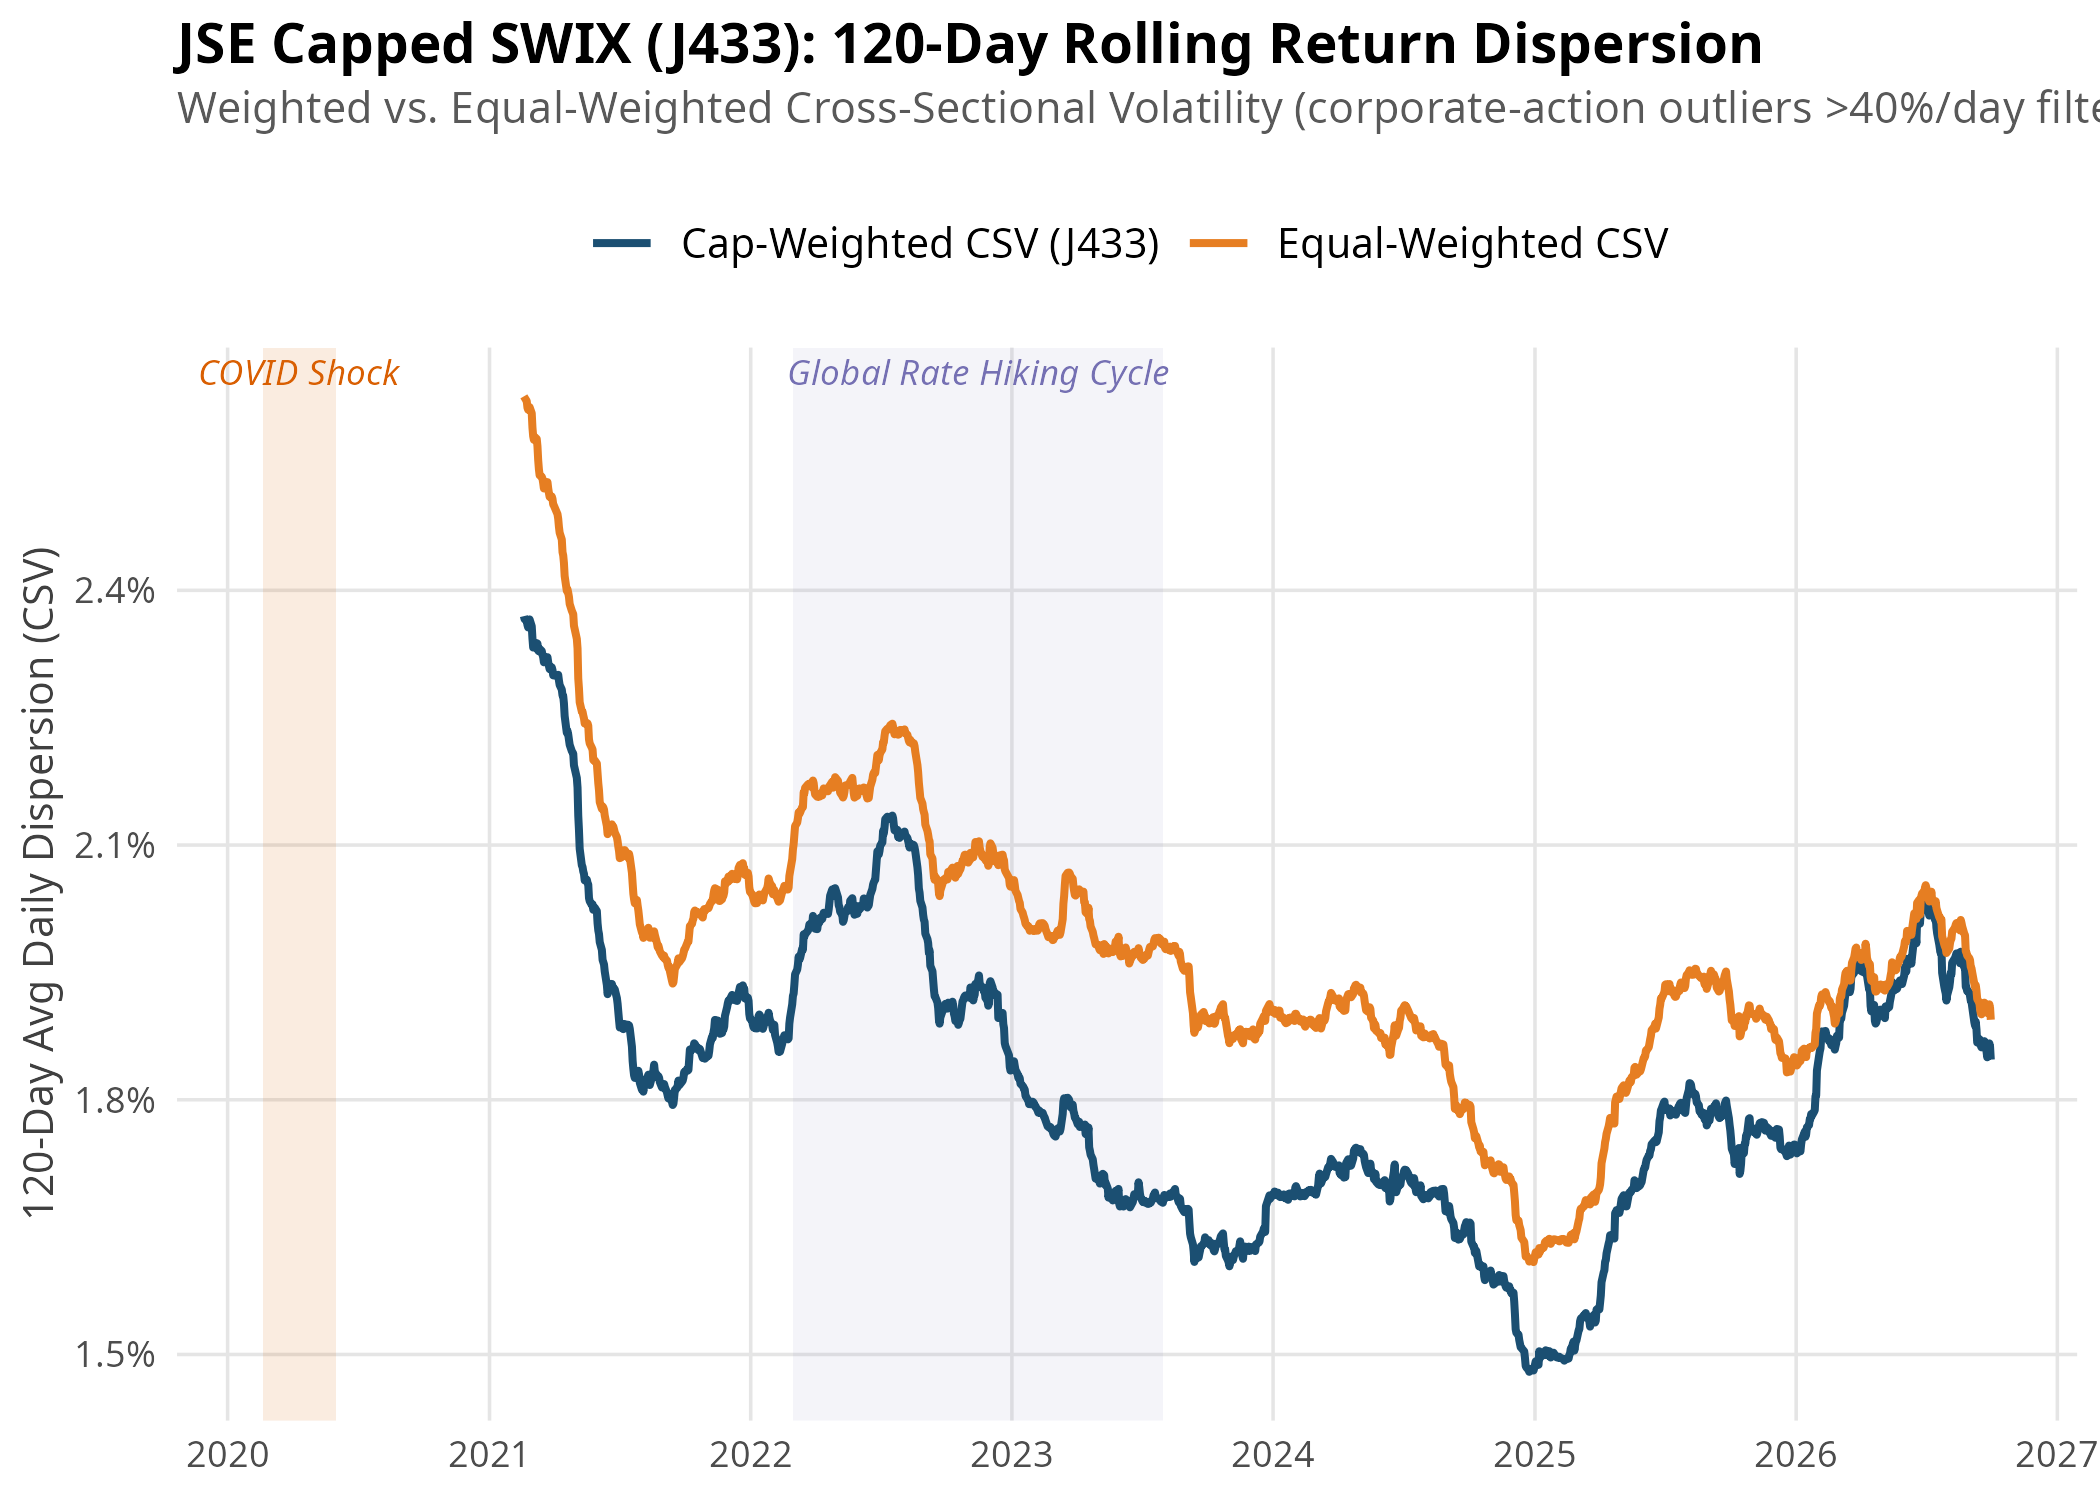
\includegraphics[width=1\linewidth]{figures/csv_dispersion_plot}

\begin{itemize}
\tightlist
\item
  Cross-sectional volatility (CSV) measures how far individual stock
  returns spread around the index on a typical day. Higher dispersion
  gives stock selection more room to add (or lose) value.
\item
  Both series fall sharply through 2021 (equal-weighted about 2.7\% to
  1.9\%, cap-weighted about 2.4\% to 1.8\%), rise during the 2022 hiking
  cycle, and reach a trough at the end of 2024 (cap-weighted about
  1.5\%).
\item
  Dispersion recovers to about 2.0\% by mid-2026, and the two measures
  converge. Large caps are now about as dispersed as the average stock.
\item
  Equal-weighted CSV is above cap-weighted CSV throughout, so smaller
  constituents have more idiosyncratic returns.
\end{itemize}

\subsection{Correlation and systemic
absorption}\label{correlation-and-systemic-absorption}

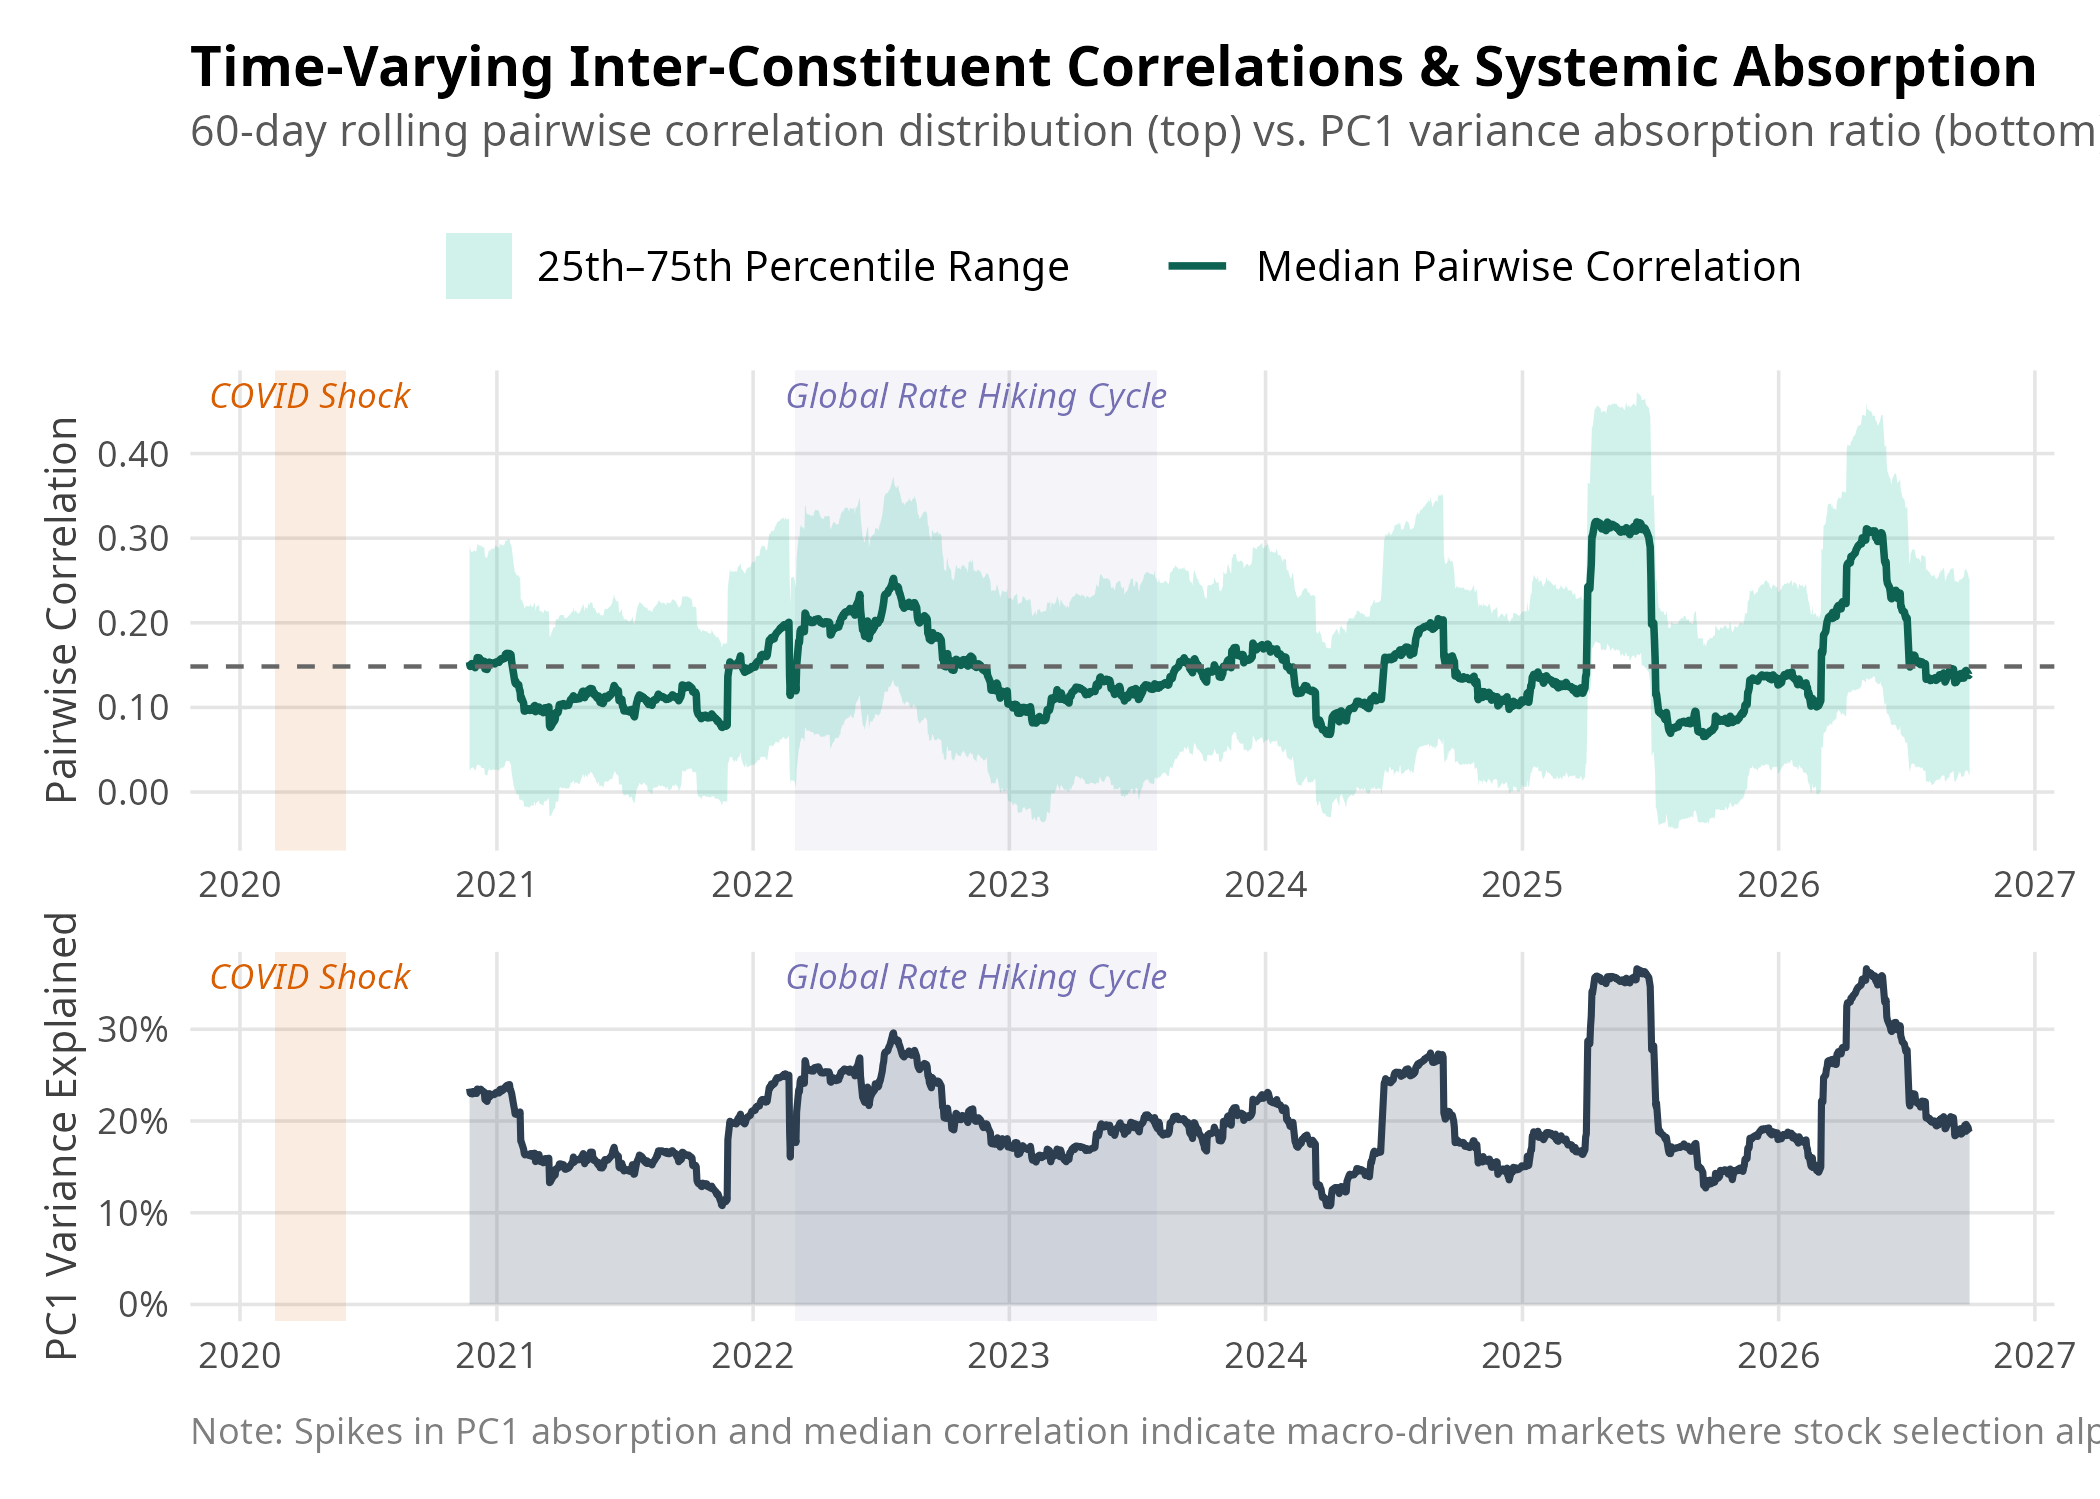
\includegraphics[width=1\linewidth]{figures/correlation_regimes_plot}

\begin{itemize}
\tightlist
\item
  Median 60-day pairwise correlation is usually 0.10--0.20, with spikes
  to about 0.25 in 2022 and above 0.30 in April--June 2025 and mid-2026.
\item
  PC1 variance absorption moves with it: typically 12--25\%, peaking at
  about 36\% in 2025 and 2026.
\item
  In these episodes stocks move together, so the market is macro-driven
  and stock selection matters less.
\end{itemize}

\subsection{Alpha-opportunity regimes}\label{alpha-opportunity-regimes}

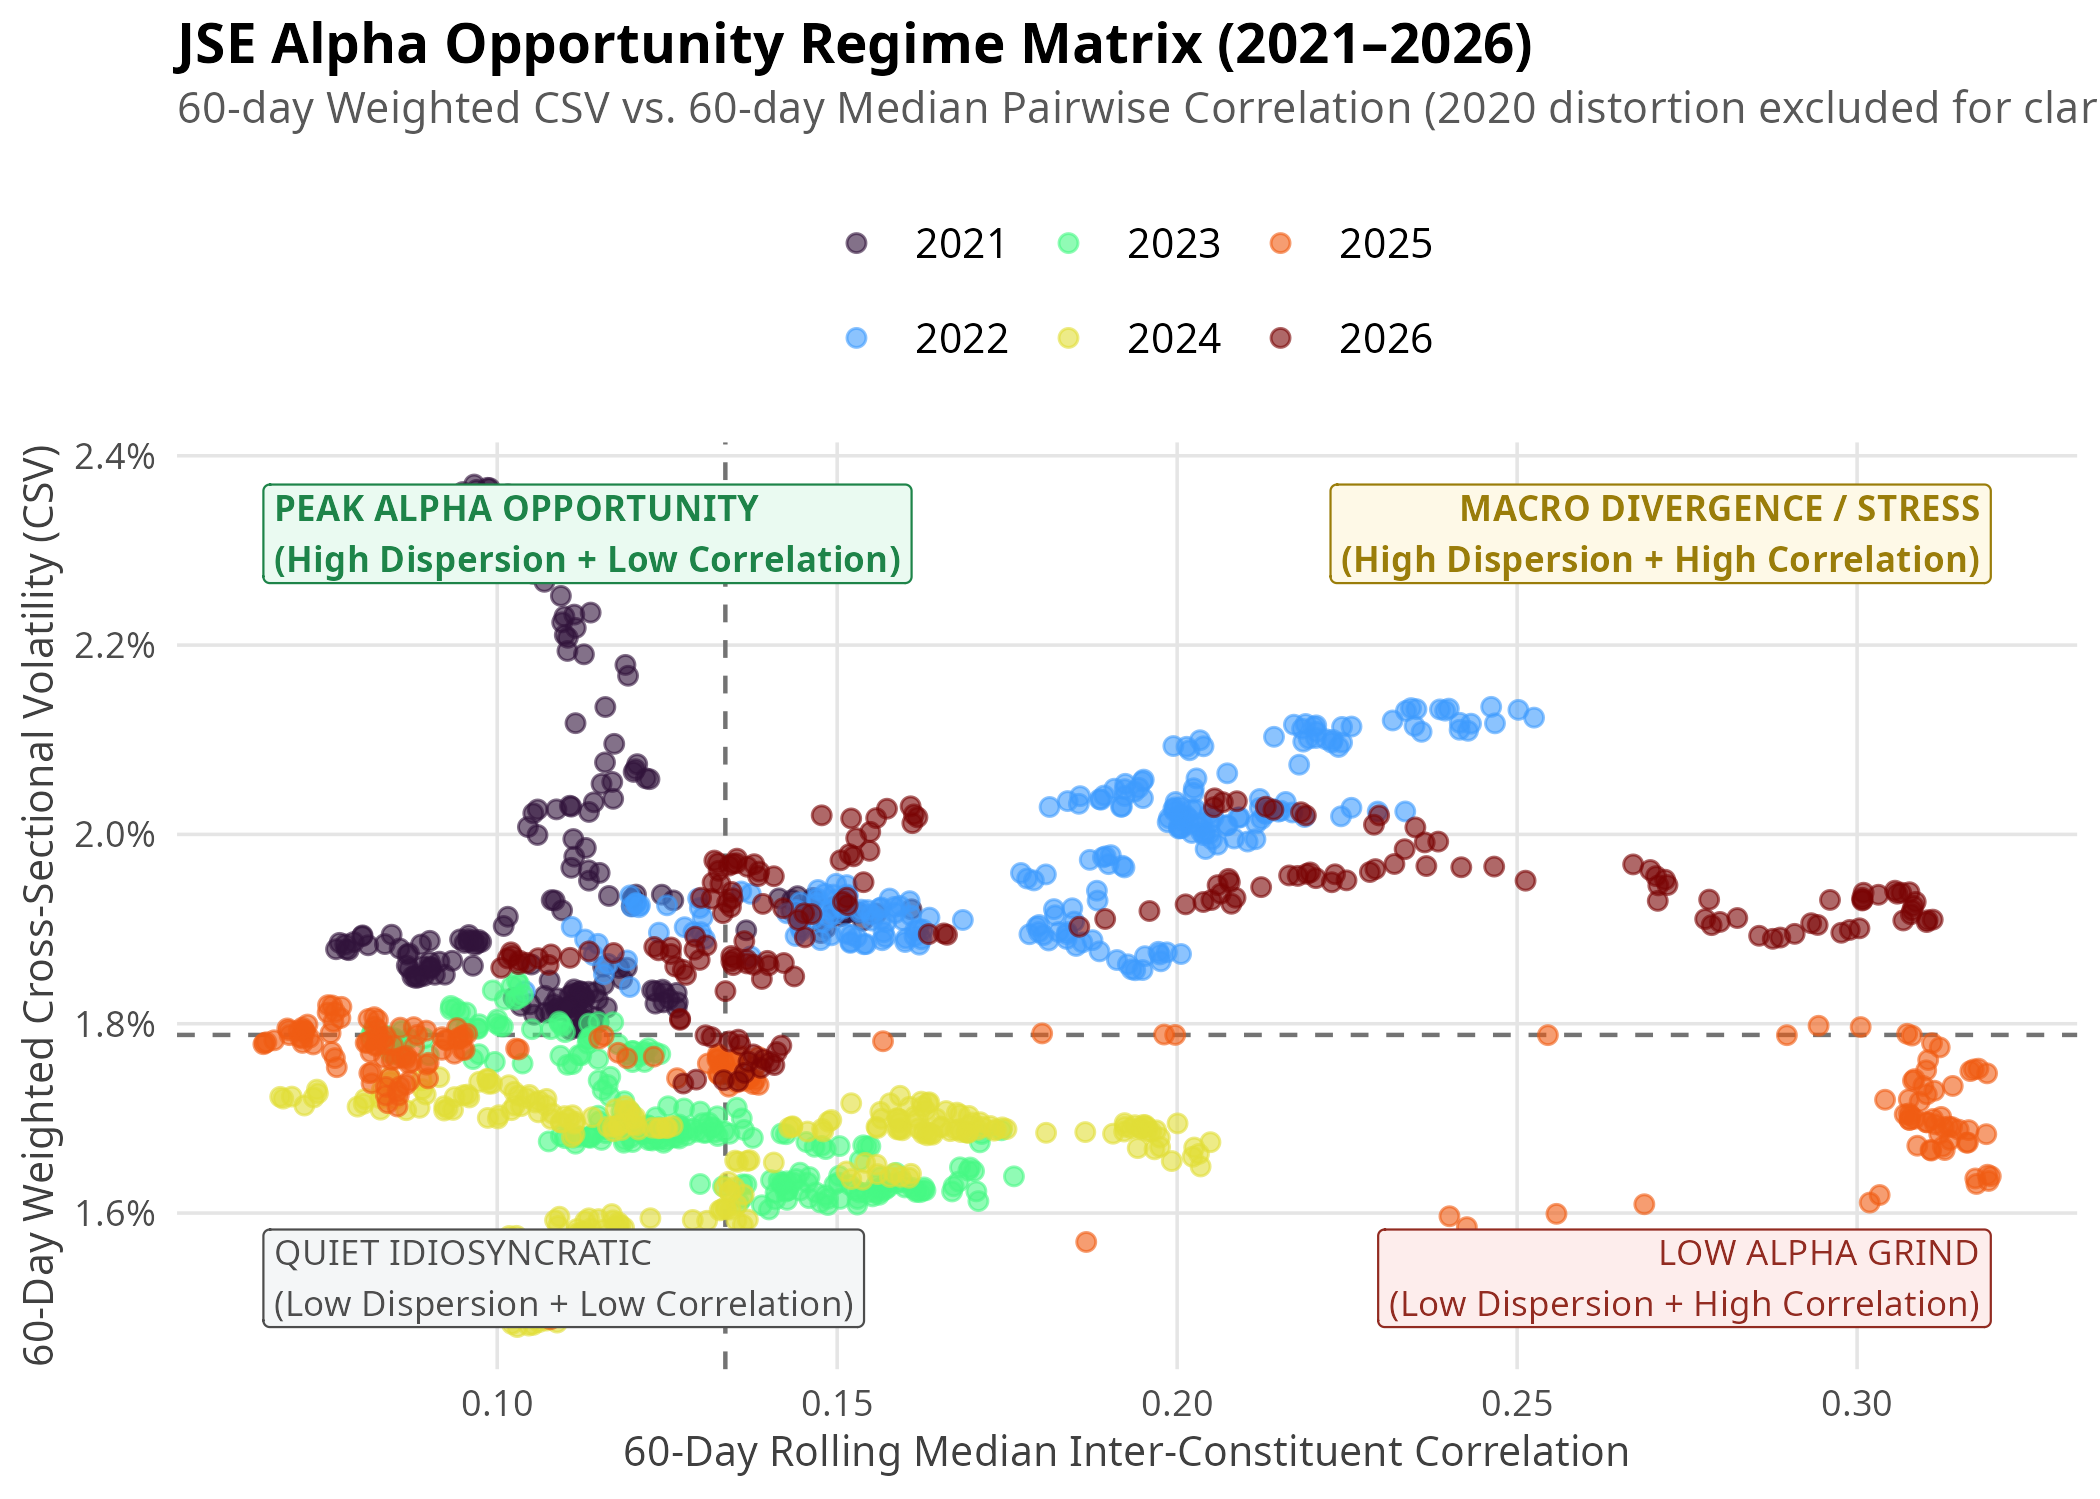
\includegraphics[width=1\linewidth]{figures/alpha_quadrant_plot}

\begin{itemize}
\tightlist
\item
  \textbf{2021:} high dispersion with low correlation (CSV up to 2.4\%,
  correlation about 0.09--0.12). This is the best environment for stock
  picking.
\item
  \textbf{2022:} high dispersion with rising correlation (about
  0.15--0.25), a macro-divergence/stress regime.
\item
  \textbf{2023--2024:} low dispersion at low to moderate correlation, a
  quiet, low-alpha period.
\item
  \textbf{2025:} mostly low dispersion, and the high-correlation points
  sit in the low-alpha quadrant.
\item
  \textbf{2026:} dispersion of about 1.9--2.0\% with correlation up to
  0.31, back in the macro-divergence/stress quadrant.
\end{itemize}

\subsection{Macro drivers}\label{macro-drivers}

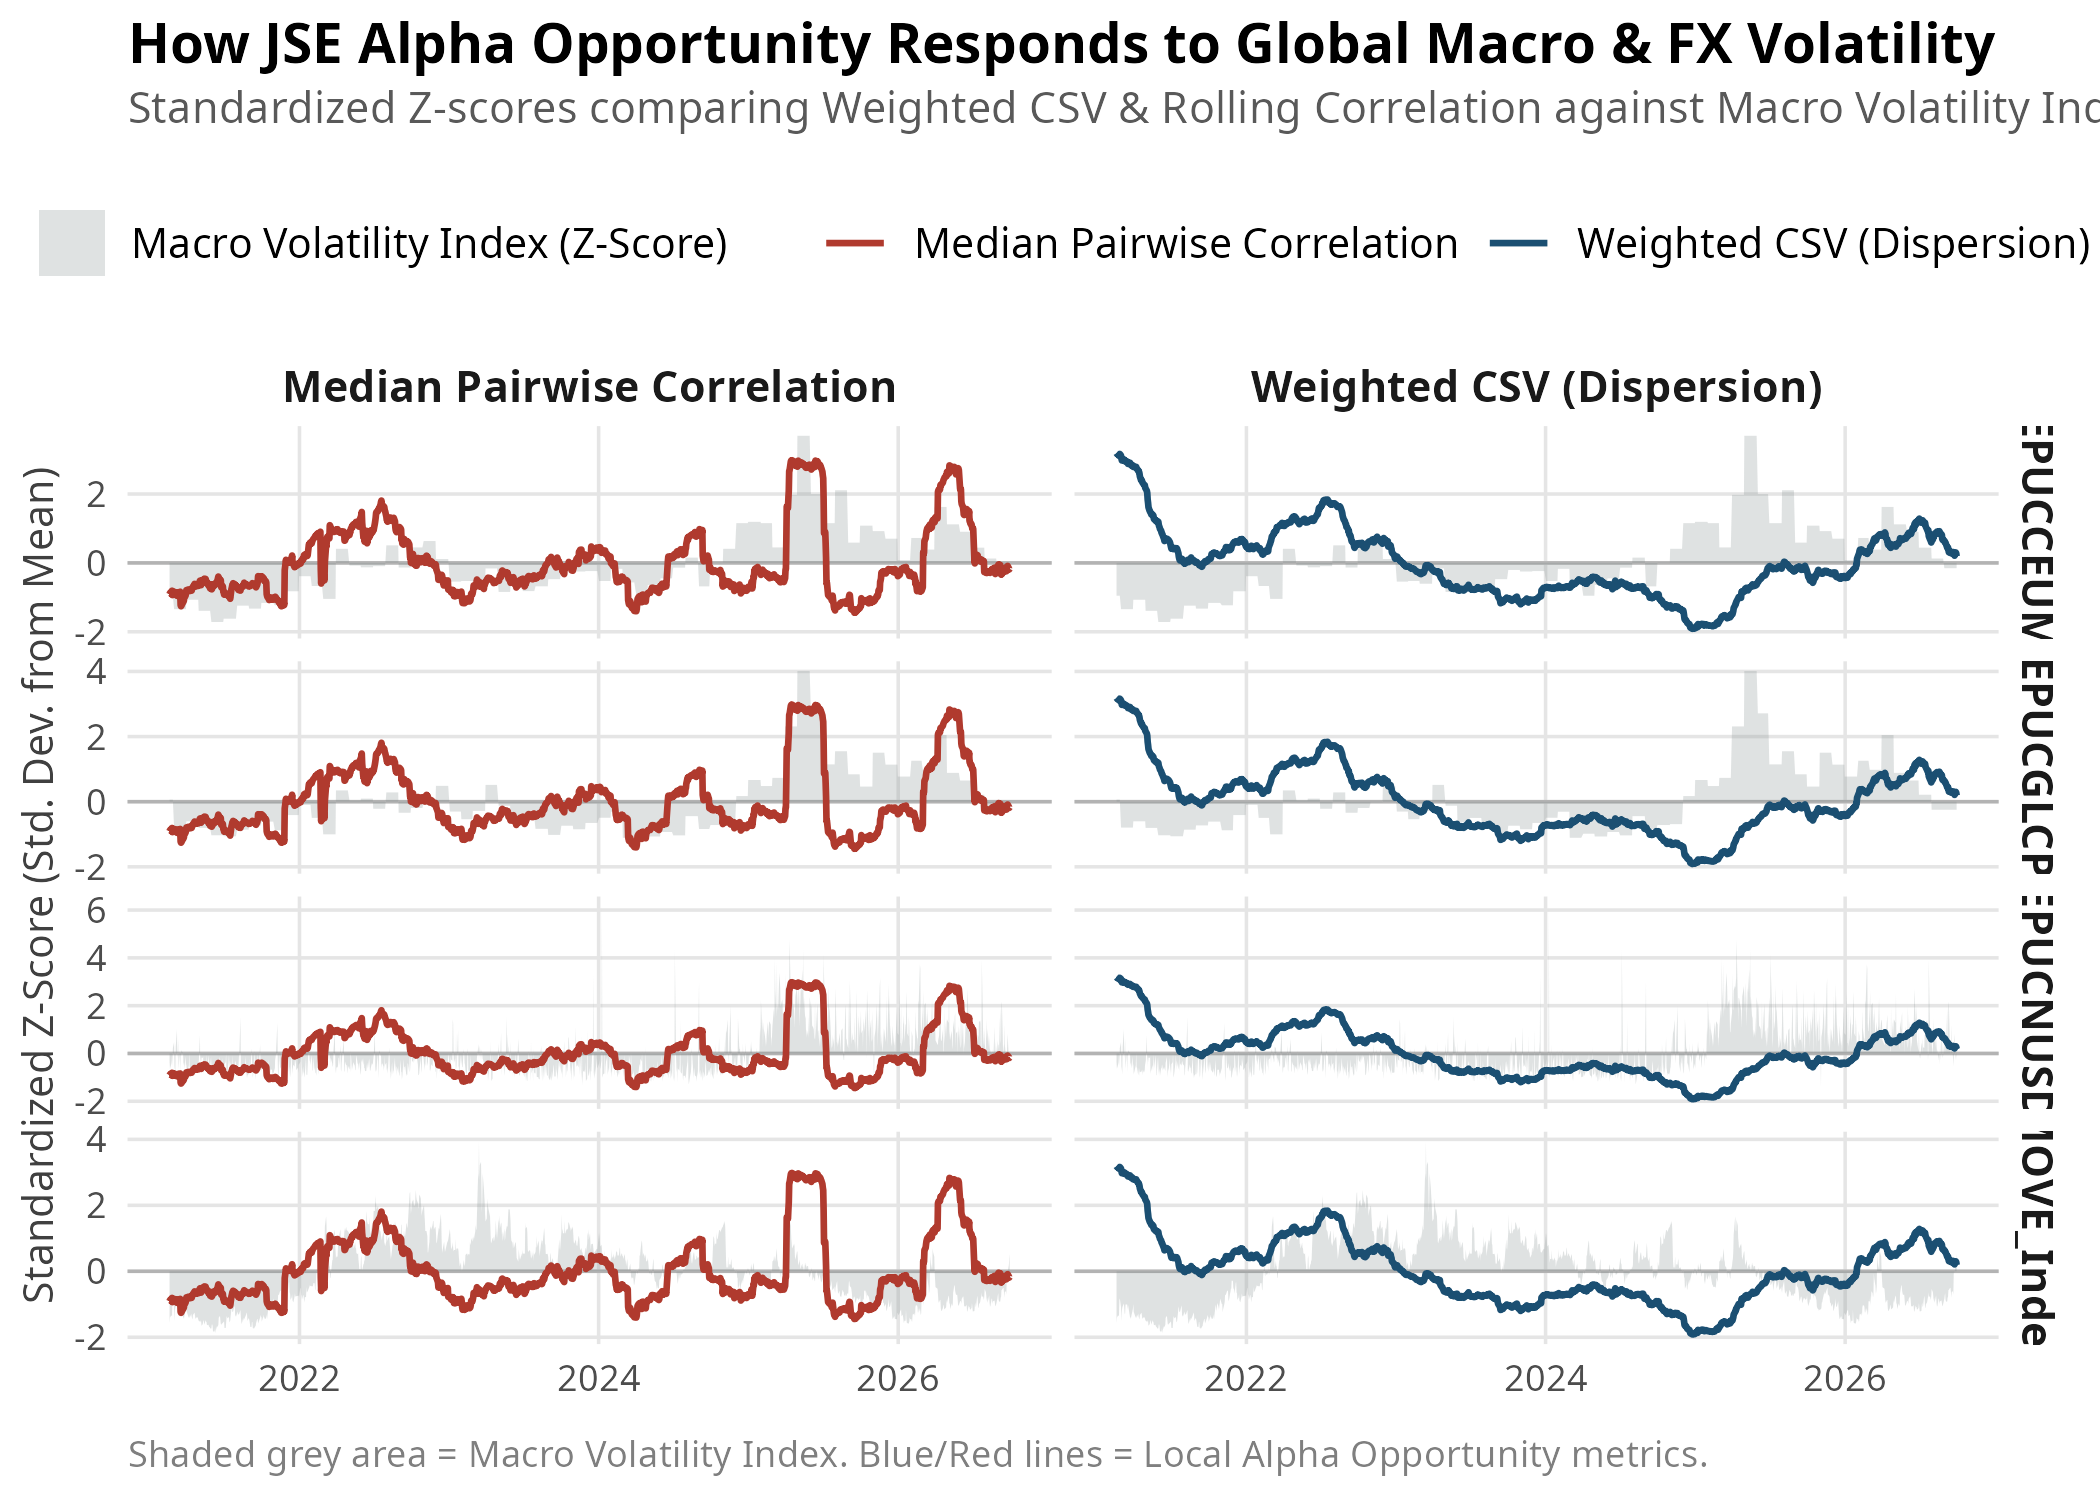
\includegraphics[width=1\linewidth]{figures/macro_drivers_plot}

\begin{itemize}
\tightlist
\item
  The 2025 and 2026 spikes in correlation line up with spikes in the
  global macro volatility indicators, but dispersion does not react in
  the same way. It was at a low in late 2024 and rose gradually.
\item
  Macro shocks therefore mostly raise co-movement rather than
  dispersion. When global macro volatility rises, stock selection has
  less to work with.
\item
  This is a visual reading, not a statistical test. A regression or
  Granger test would be needed to confirm it.
\end{itemize}

\subsection{. Implications}\label{implications}

\begin{itemize}
\tightlist
\item
  The opportunity for stock selection is regime-dependent. It is highest
  when correlation is low and dispersion high (2021), and lowest in
  macro-driven markets (2025--26 spikes).
\item
  This is consistent with Part B: SafeCore tracks the Capped SWIX
  closely, so in macro-driven periods there is little to diversify with.
\item
  If volatility management is a goal, risk limits (stock and sector risk
  budgets, ENB monitoring) matter most when correlations spike.
\end{itemize}

\bibliography{Tex/ref}





\end{document}
